\documentclass[a4paper, openright, twosides]{book}
\usepackage{geometry}
\geometry{hmargin={3cm,3cm},vmargin={3cm,3cm}}
\usepackage[english,italian]{babel}
\usepackage[T1]{fontenc}
\usepackage[utf8]{inputenc}
\usepackage{fancyhdr}
\usepackage{float}
\usepackage{graphicx}
\usepackage{wrapfig}
\usepackage{siunitx} %per scrivere il simbolo °
\usepackage{verbatim} %per i commenti1
\usepackage{subfig}
\usepackage{amsmath}
\usepackage[linesnumbered, ruled, vlined]{algorithm2e}
\usepackage{algorithmic}
\setcounter{secnumdepth}{3}
\setcounter{tocdepth}{6}
\usepackage{multirow}
\newcommand{\minitab}[2][l]{\begin{tabular}#1 #2\end{tabular}}
\usepackage{rotating}
\usepackage{xfrac}
\usepackage{enumitem}
\usepackage{amsmath}
\usepackage{showlabels}
\usepackage{cases}

\DeclareMathOperator*{\argmax}{arg\,max}
\DeclareMathOperator*{\argmin}{arg\,min}

%\usepackage{booktabs,array}
%\usepackage{tikz}

%\usepackage{tabularx}

%\usepackage{chngcntr}
%\counterwithin{table}{section}

%------------------------------ colors
\usepackage[usenames,dvipsnames,table]{xcolor} % use colors on table and more
\definecolor{333}{RGB}{51, 51, 51} % define custom color
\definecolor{background}{RGB}{255, 254, 213}
\definecolor{comment}{RGB}{17,167,5}
\definecolor{keyword}{RGB}{195,47,8}
\definecolor{string}{RGB}{142,195,0}
\definecolor{number}{RGB}{90,84,84}
\definecolor{identifier}{RGB}{0,90,201}

%------------------------------ source code
\usepackage{listings}

\lstset{
  basicstyle=\footnotesize\sffamily,
  commentstyle=\itshape\color{gray},
  captionpos=b,
  frame=shadowbox,
  language=HTML,
  rulesepcolor=\color{333},
  tabsize=2
}

\lstdefinestyle{code}{
  backgroundcolor=\color{background},
  basicstyle=\footnotesize\sffamily,
  commentstyle=\color{comment},
  frame=L,
  identifierstyle=\color{identifier},
  keywordstyle=\color{keyword},
  numbers=left,
  numbersep=10pt,
  numberstyle=\tiny\color{number},
  stringstyle=\color{string},
  showstringspaces=false,  
  stepnumber=1,
  tabsize=2
}


%------------------------------ define Abstract environment, missing in the 'book' class
\newenvironment{abstract}{\cleardoublepage \null \vfill \begin{center}\bfseries\abstractname \end{center}}{\vfill\null}
\addto\captionsenglish{\renewcommand*\abstractname{Abstract}} % change Abstract title

%------------------------------ active url
\usepackage{url}
\renewcommand{\UrlFont}{\color{black}\small\ttfamily}
\usepackage[colorlinks=true, linkcolor=black, citecolor=black, urlcolor=black]{hyperref} % active ref
%------------------------------ macros
\newcommand{\sectionname}{Section} % define Section ref
\newcommand{\subsectionname}{Sub-section} % define Sub-section ref
\renewcommand*\arraystretch{1.4} % tables padding

%acronimi
\usepackage[printonlyused]{acronym}

\begin{document}
\frontmatter

\begin{titlepage} %------------------------------ TITLE PAGE
\begin{center}

\hspace{0.5cm}
\begin{minipage}{.20\textwidth}
  
\includegraphics[height=2.5cm]{Images/UNIPD}
\end{minipage}\begin{minipage}{.90\textwidth}
  \begin{table}[H]
  \begin{tabular}{l}
  \scshape{\Large{\bfseries{Università degli Studi di Padova}}} \\
  \hline \\
  \scshape{\Large{Facoltà di Ingegneria}} \\
  \end{tabular}
  \end{table}
\end{minipage}

\vspace{1cm}
\emph{\Large{Corso~di~Laurea~Magistrale~in~Ingegneria~Informatica}} \\
\vspace{3cm}
\scshape{\Large{Tesina di Ricerca Operativa 2}} \\
\end{center}

\vspace{1cm}
\begin{center}
\scshape{\Large{\bfseries{Travelling Salesman}}}\\
\scshape{\Large{\bfseries{Problem}}}
\end{center}

\vspace{3.5cm}

\begin{center}
\emph{Autori}
\vspace{0.2cm}
\begin{table}[h]
\centering
\begin{tabular}{rl}
\vspace{0.2cm}
{Raffaele Di Nardo Di Maio} & {1204879}\\
{Cristina Fabris} & {1205722}\\
\end{tabular}
\end{table}

\end{center}

\vfill
\begin{center}
\hspace{-0.2cm}
\line(1, 0){360}\\
\textsc{Anno Accademico 2019-2020}
\end{center}
\end{titlepage}

%\begin{comment}
\begingroup %------------------------------ CONTENTS
  \makeatletter
  \let\ps@plain\ps@empty
  \makeatother
  \tableofcontents  
  \clearpage
\endgroup
%\end{comment}

\begin{comment}
\makeatletter %REMOVE Chapter Title in each chapter but not in the index
\def\@makechapterhead#1{%
  \vspace*{50\p@}%
  {\parindent \z@ \raggedright \normalfont
    \vskip 20\p@
    \interlinepenalty\@M
    \Huge \bfseries #1\par\nobreak
    \vskip 40\p@
  }}
\makeatother
\end{comment}

\mainmatter
\chapter{Introduzione}\label{intro}
La seguente trattazione analizza il Problema del Commesso Viaggiatore (Travelling Salesman Problem, TSP), che consiste nell'individuare un circuito hamiltoniano di costo minimo in un assegnato grafo orientato G=(V,A)\cite{TSP}. La formulazione matematica di tale problema è la seguente:
$$
x_{ij}=
\begin{cases}
1 & se\;l'arco\;(i,j)\in A\;viene\;scelto\;nel\;circuito\;ottimo\\
0 & altrimenti\\
\end{cases}
$$
\begin{align}
& min \underset{(i,j)\in A}\sum{c_{ij}\;x_{ij}} \\\notag \\
& \underset{(i,j)\in \delta^{-}(j)}\sum{\;x_{ij}} = 1 & \forall\;j\in V \\\notag \\
& \underset{(i,j)\in \delta^{+}(i)}\sum{\;x_{ij}} = 1 & \forall\;i\in V \\\notag \\
& \underset{(i,j)\in \delta^{+}(S)}\sum{\;x_{ij}} \geq 1 & S \subset V\; :\; 1\in S\\\notag \\
& x_{ij}\geq 0\;\; intero & (i,j)\in A.\\\notag
\end{align}
Tuttavia le soluzioni algoritmiche presentante risolvono una sua variante, detta simmetrica, che viene applicata ad un grafo completo non orientato G=(V,E).\\ Di seguito viene riportata la formulazione matematica di tale versione:\\
\begin{align}
& min \underset{e\in E}\sum{c_e\;x_e}\\
& \underset{e\in \delta(v)}\sum{\;x_e} = 2 & \forall\;v\in V \\
& \underset{e\in E(S)}\sum{\;x_e} \leq \vert S\vert - 1 & \forall\;S\underset{\neq} \subset V: \vert S\vert\geq 3.\\\notag
\end{align}
A livello commerciale esistono diverse tipologie di risolutori di problemi di programmazione lineare intera, basati sul Branch \& Bound. I più conosciuti in circolazione sono i seguenti:
\begin{itemize}
\item{\textbf{IBM ILOG CPLEX Optimization Studio}\cite{ILOG}\\
è un soluzione analitica, sviluppata dall'IBM e gratuita a livello accademico.}
\item{\textbf{FICO® Xpress Optimization}\cite{FICO}\\
è stato prodotto dalla Fair Isaac Corporation(FICO) ed è costituito da 4 componenti principali: FICO® Xpress Insight, FICO® Xpress Executor, FICO® Xpress Solver e FICO® Xpress Workbench. Questa soluzione è disponibile gratuitamente solo nella versione Community, in cui però vengono applicate restrizioni sul numero di righe e colonne del tableau, di token non lineari e di funzioni dell'utente.}
\item{\textbf{Gurobi}\cite{GUROBI}\\
è una soluzione, sviluppata dalla Gurobi Optimization, che viene rilasciata anche con una versione accademica.}
\item{\textbf{COIN Branch and Cut solver (CBC)}\cite{CBC}\\
è un risolutore MIP(mixed-integer program) open-source scritto in C++ e sviluppato dalla Computational Infrastructure for Operations Researc (COIN).}
\end{itemize}
Nel Capitolo \ref{CPLEX} vengono riportate diverse soluzioni mat-euristiche e non per il problema del Commesso Viaggiatore, che fanno uso di ILOG CPLEX.\\
In commercio, il più noto ed efficiente software per la risoluzione del TSP è Concorde, sviluppato in ANSI C e disponibile per l'uso in ambito accademico\cite{concorde}.\\
Nel Capitolo \ref{HEURISTIC} vengono analizzati gli algoritmi euristici, sviluppati senza far uso di ILOG CPLEX.\\
Nel Capitolo \ref{PERF_PROF} vengono invece riportati i confronti, a livello temporale e di costo, delle soluzioni ottenute con i differenti algoritmi enunciati.\\
Nell'Appendice \ref{TSPlib}, \ref{CPLEX_func}, \ref{gnuplot}, \ref{perf_profile_py} vengono descritte rispettivamente la tipologia di istanze utilizzate, la documentazione utilizzata ed il funzionamento di CPLEX, il programma GNUPLOT utilizzato nella stampa delle soluzioni e il programma perfprof.py usato per creare i performance profile del Capitolo \ref{PERF_PROF}.\\
Tutti i tempi di esecuzione e i costi delle soluzioni, ottenuti mediante la fase di testing, sono consultabili invece nelle tabelle riportate nell'Appendice \ref{results}. Tutte le soluzioni descritte sono state implementate in linguaggio C e testate sul sistema operativo Windows 10 con Visual Studio, ed i sorgenti sono disponibili online\footnote{\url{https://github.com/RaffaDNDM/Operational-Research-2}}.
\chapter{Risoluzione del problema tramite CPLEX}\label{CPLEX}  

\section{Modelli compatti}
I modelli compatti del Travelling Salesman Problem, sono formulazioni matematiche in cui il numero di variabili e di vincoli è polinomiale nella taglia dell'istanza. In particolare, in quelle analizzate in seguito,esse sono entrambe $O(n^2)$, con \textit{n = numero di nodi}.\\
I modelli compatti sono però applicabili solo a grafi orientati. Quindi ciascuna variabile $x_{ij}$ del modello simmetrico deve essere convertita nelle due variabili $x_{ij}$ e $x_{ji}$ del corrispondente modello orientato (vedi Capitolo \ref{intro}). Questo comporta un significativo rallentamento nella computazione della soluzione, in quanto il metodo di risoluzione, nel momento in cui si trovi a scartare un ramo $(i,j)$ dalla possibile soluzione, deve verificare comunque se il corrispondente lato $(j,i)$ potrebbe invece farne parte. Tale controllo risulta però inutile, poichè i due rami vengono associati alla stessa variabile nel modello simmetrico iniziale.
Entrambi i modelli descritti in questa sezione sono stati sviluppati ed il confronto dei tempi di esecuzione delle relative implementazioni viene riportato nella Sezione \ref{compact_perf}.

\subsection{Formulazione di Miller, Tucker e Zemlin}
Nella formulazione del modello di Miller, Tucker e Zemlin, detta anche formulazione sequenziale, per ogni nodo \textit{i} del grafo viene introdotta una nuova variabile $u_i$ , che rappresenta la posizione di tale vertice all'interno del circuito restituito. Vengono introdotti inoltre nuovi vincoli basati sulle variabili $u_i$ che garantiscono la formazione di un unico tour e l'eliminazione di tutti i possibili subtour.\\
Nello specifico il modello utilizzato da Miller, Tucker e Zemlin è il seguente:
\vspace{1cm}
\begin{align}
& min \underset{i\in V}\sum{}\underset{j\in V}\sum{c_{i,j}\; x_{i,j}} \\ \notag \\
& \underset{i\in V}\sum{x_{ih}}\; =\; 1 & \forall\; h\in V \\ \notag \\
& \underset{j\in V}\sum{x_{hj}}\; =\; 1 & \forall\; h\in V \\ \notag \\
& u_i-u_j+n\; x_{i,j}\;\leq\; n-1 & \forall\; i,j\in V-\{ 1\} , i\neq j \\ \notag \\
& 0\leq u_i\;\leq\; n-2 & \forall\; i\in V-\{ 1\} \\ \notag 
\end{align}
Esistono però due diversi modi per inserire i vincoli aggiuntivi, sfruttando le funzioni di CPLEX.\\
Nel primo questi vengono aggiunti direttamente al modello, durante la costruzione di quest'ultimo. In tal modo, durante la fase di preprocessamento, il programma è già a conoscenza di tutti i vincoli che dovrà rispettare la soluzione ottima e ciò gli permette di apportare ulteriori semplificazioni al modello, rilevandone alcune proprietà utili.\\
Il secondo metodo, invece, prevede l'inserimento nel modello di questi vincoli tramite "lazy constraint". In tal modo i vincoli non sono noti al programma dall'inizio, ma vengono inseriti all'interno di un pool. Nel momento in cui viene calcolata una soluzione, CPLEX ne verificarà la correttezza analizzando l'insieme di vincoli precedentemente definito e se dovesse trovarne uno violato, lo aggiunge al modello e ripete la computazione.\\
Questo secondo approccio implementativo permette di eseguire calcoli su un modello di dimensioni inferiori rispetto a quello ottenuto utilizzando il primo metodo. Tuttavia i tempi di calcolo possono aumentare significativamente in quanto CPLEX non può sfruttare la conoscenza dell'intero modello sin dalla sua costruzione. 
Nell'implementazione sviluppata, sono state impiegate entrambe le soluzioni descritte.

\subsection{Formulazione di Gavish e Graves}
Nella formulazione di Gavish e Graves, per impedire la formazione di sub-tour all'interno della soluzione, viene associata a ciascun ramo una nuova variabile $y_{ij}$, che rappresenta il flusso tra i nodi $i$ e $j$. Il modello, legato al problema del commesso viaggiatore, assume la seguente forma:
\begin{align}
& min\underset{i\in V}\sum{\underset{j\in V}\sum{c_{i,j}\; x_{ij}}} \\ \notag \\
& \underset{i\in V}\sum{x_{ih}}\;=\;1 & \forall\;h\in V \\ \notag\\
& \underset{j\in V}\sum{x_{hj}}\;=\;1 & \forall\;h\in V \\ \notag\\
& \underset{j\in V}\sum{y_{1j}}\;=\;n-1\\ \notag\\
& \underset{j\in V}\sum{y_{hj}}\;=\;\underset{i\in V}\sum{y_{ih}}\;-1 & \forall\;h\in V-\{1\}\\ \notag\\
& y_{ij}\leq\;(n-1)\;x_{ij} & \forall\;i,j\in V, i\neq j\\ \notag
& y_{ii}=0 & \forall\;i\in V\\\notag
& y_{i1}=0 & \forall\;i\in V\\\notag
\end{align}
In questo formulazione matematica, i vincoli di subtour elimination vengono sostituiti dai vincoli $(2.9)$, $(2.10)$, $(2.11)$, $(2.12)$, $(2.13)$ che rappresentano rispettivamente: il flusso di uscita dal primo nodo, il bilanciamento dei flussi in ogni singolo nodo, i vincoli di accoppiamento del flusso con un ramo selezionato nella soluzione, il valore del flusso su auto-anelli e il valore del flusso entrante nel primo nodo.\\
La soluzione di questo modello risulta essere però molto lontana dalla convex hull e per migliorarla è possibile sostituire il vincolo \textit{(2.11)} con: \\
\begin{center}
$y_{ij}\leq\;(n-2)\;x_{ij} \;\;\;\;\;\forall\; i\neq \; j$.\\
\end{center} 
Inolte per evitare che la soluzione ottima imposti ad $1$ entrambi gli archi orientati $x_{i,j}$ e $x_{j,i}$, che nell'istanza iniziale sono legati allo stesso arco, viene aggiunto anche il seguente vincolo:
\begin{center}
$x_{i,j}+x_{j,i}\leq 1\;\;\;\; \forall i,j \in V$ con $i < j$
\end{center}
L'implementazione svolta all'interno del programma utilizza i vincoli $(2.11)$ nella sua prima forma e li inserisce nel modello in fase di costruzione.

\section{Algoritmi Esatti}
\subsection{Loop}
Negli anni '60, Jacques F. Benders sviluppò un approccio generale, applicabile a qualsiasi problema di programmazione lineare, per ridurre il numero esponenziale di vincoli presenti in un modello.\\
Per risolvere tale problema, il metodo loop costruisce inizialmente il modello senza quei vincoli e li aggiunge solo in seguito durante la risoluzione del problema. Il metodo di Benders calcola una soluzione e valuta se questa rispetti tutti i vincoli non inseriti nel modello.\\
Nel caso in cui l'algoritmo dovesse trovarne uno che non viene rispettato, lo inserisce nel modello. 
Nel caso del TSP, i vincoli in numero esponenziale sono i Subtour Elimination, che hanno la seguente forma:
\begin{align}
&\underset{e\in E(S)}\sum{x_{e}} \leq \mid S\mid - 1\;\forall\;S\underset{\neq}{\subset}V\; : \; \mid S\mid\geq 2
\end{align}
o equivalentemente:
\begin{align}
&\underset{e\in \delta(S)}\sum{x_{e}}\geq 2\;\forall\;S\underset{\neq}{\subset}V\; : \; \mid S\mid\geq 2
\end{align}
Definendo il modello per problema del commesso viaggiatore, vengono rimossi i vincoli di Subtour ELimination. In seguito viene risolto il problema e nel caso in cuila soluzione abbia più di una componente connessa, viene aggiunto al modello un vincolo di subtour elimination per ogni 
ciclo generato. Il processo viene ripetuto iterativamente, come mostrato nel seguente pseudocodice, fino a che la soluzione non sia costituita da un unico tour.\\\\
\begin{algorithm}[H]
\DontPrintSemicolon
\KwIn {$\mathtt{model}$= Modello TSP simmetrico senza vincoli di Subtour Elimination\newline}
\KwOut {$\mathtt{x}$= soluzione intera senza subtour}
\BlankLine 
 $\mathtt{x} \gets$ solve(model)\;
 $\mathtt{ncomps} \gets$ comps(x)\;
 \BlankLine 
 \While{$\mathtt{ncomps} \geq 2$}{
  Aggiungi $\underset{e\in \delta(S_k)}\sum{x_{e}}\leq \mid S_k\mid - 1\;\forall$ componente connessa $S_k$\;
  \BlankLine  
  \If{$\mathtt{ncomps} \geq 2$}{
    \BlankLine
    $\mathtt{x} \gets$ solve(model)\;
    $\mathtt{ncomps} \gets$ comps(x)\;
  }
 }
 \caption{LOOP}
\end{algorithm}
All'aumentare del numero di vincoli inseriti nel modello, il costo della soluzione peggiora o resta invariato rispetto al costo di quella elaborata all'iterazione precedente del metodo loop.\\
Il numero di iterazioni che vengono effettuate dall'algoritmo non è calcolabile a priori e potrebbe essere anche molto elevato. Nel caso peggiore verranno inseriti tutti i vincoli di Subtour elimination, ovvero un numero esponenziale di disequazioni, soprattutto nel caso di istanze clusterizzate.\\
L'introduzione di nuovi vincoli di Subtour Elimination, solo nel momento in cui si presenta una loro violazione, permette di ridurre la dimensione del modello ma riduce l'attività di pre-processamento svolta da CPLEX prima di risolvere il problema.
Inoltre il problema principale del metodo loop è la generazione di un nuovo albero completo di branching ad ogni iterazione del loop.\\
In passato, con le versioni del MIP solver di CPLEX, questa operazione era molto onerosa mentre attualmente il metodo loop garantisce la risoluzione, anche di istanze molto grandi, in tempi ragionevoli.
Questo non accade invece per il Branch \& Bound in quanto vengono aggiunte nuove ramificazioni all'albero già esistente.\\
Il metodo loop può essere modificato svolgendo prima l'algoritmo loop con l'aggiunta di parametri differenti da quelli utilizzati di default del risolutore CPLEX e solo in seguito viene effettuato l'algoritmo di Benders ma questa volta utilizzando le impostazioni di default di CPLEX. \\
Quest'ottimizzazione è basata sul fatto che CPLEX salvi alcune soluzioni, ottenute in precedenza dal risolutore sullo stesso modello, e le sfrutti come bound nel nuovo modello. Per questo motivo, la soluzione metaeuristica ottenuta nella prima fase viene sfruttata come bound nella seconda.

\subsection{Branch \& Cut}
Come precedentemente anticipato, CPLEX effettua inizialmente una fase di pre-processamento in cui semplifica il modello, e terminata questa operazione inizia ad eseguire la fase di Branch \& Cut. Ogni volta che calcola una nuova soluzione $x^*$, prima di dichiarare se è l'ottimo o di scartarla e proseguire a sviluppare i successivi rami dell'albero decisionale, applica dei tagli e degli algoritmi euristici per aggiornarla (vedi Figura \ref{Albero_decisionale}).
\begin{figure}[h] 
\begin{center} 
  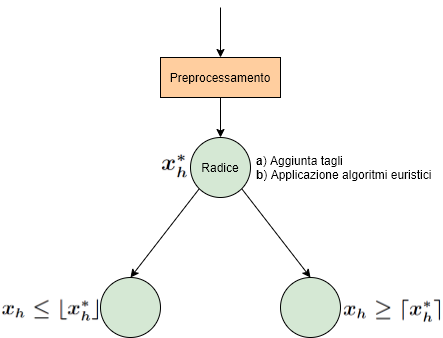
\includegraphics[scale=0.7]{Images/albero_decisionale}\\ 
  \caption{\footnotesize{Albero decisionale del Branch and Cut}}
  \label{Albero_decisionale} 
\end{center} 
\end{figure}
Nello sviluppo del Branch \& Cut, per ciascun nodo dell'albero decisionale, vengono considerati due bound:
\begin{itemize}
\item{\textbf{Upper Bound}\\
viene definito dagli algoritmi euristici utilizzati.
}
\item{\textbf{Lower Bound}\\
viene definito dal rilassamento del problema.
}
\end{itemize}
CPLEX permette di personalizzare i tagli da applicare nel Branch \& Cut e inserendo iterativamente i Subtour Elimination relativi alle componenti connesse nella soluzione a cui verrà applicato il taglio. Per fare ciò CPLEX permette all'utente di implementarne questi vincoli mediante delle callback, \textit{lazy constraints callback}, utilizzate per aggiungere lazy constraints al modello.\\
Le callback implementate vengono chiamate solo nel momento in cui deve essere aggiornato l'incumbent e se necessario aggiunge al modello i vincoli violati. Verrà quindi invocata più frequentemente all'inizio del calcolo della soluzione del problema, e meno nelle iterazioni successive. Questo poichè essendoci in partenza meno vincoli, sarà più facile per la soluzione soddisfarli tutti.\\
A differenza dei \textit{lazy constraint}, con l'utilizzo delle \textit{lazy callback} i vincoli non sono costantemente presenti in un pool, ma vengono generati "al volo" al momento necessario.  Quest'operazione velocizza notevolmente il calcolo della soluzione ottima, in quanto permette a CPLEX di non dover calcolare nuovamente l'albero decisionale dalla radice, ma di procedere nel suo sviluppo aggiungendo nuovi rami.\\
In particolari casi, però, CPLEX può ritenere più conveniente distruggere l'intero albero decisionale finora calcolato e ricominciare la computazione dalla radice. Questo può avvenire in qualunque punto dell'elaborazione della soluzione ottima e utilizzando istanze abbastanza grandi, diventa evidente visiando i log di CPLEX.\\
Attraverso l'utilizzo delle callback è possibile accedere però a numerose informazioni relative alle elaborazioni fatte da CPLEX. Per questo motivo, alcune procedure vengono automaticamente disattivate, affinché l'utente non possa venire a conoscenza di particolari dettagli implementativi.\\
%Riascoltalo, descrivi il dynamic search
La procedura più importante che viene bloccata è il dynamic search.
Per evitare questo è possibile installare le callbacks con una modalità leggermente diversa, attraverso funzioni dette \textit{general}.

\subsection{Patching algorithm}
Negli algoritmi analizzati nei precedenti capitoli può succedere che CPLEX, prima di restituire la soluzione ottima, computi soluzioni con più componenti connesse. Per evitare che vengano scartate senza essere sfruttate   è possibile utilizzare questo semplice algoritmo euristico che si pone l'obbiettivo di convertirle in una soluzione ammissibile.\\
Date due componenti connesse all'interno della soluzione calcolata, queste vengono unite in una sola grazie all'eliminazione di un ramo ciascuna $\{a, a'\}$ e  $\{b, b'\}$ e alla selezione di altri due rami che fungano da collegamento tra i quattro vertici selezionati ($\{a, b\}$ e $\{a', b'\}$ o $\{a, b'\}$ e $\{a', b\}$) (vedi figura \ref{patching}). 
\begin{figure}[h] 
\begin{center} 
  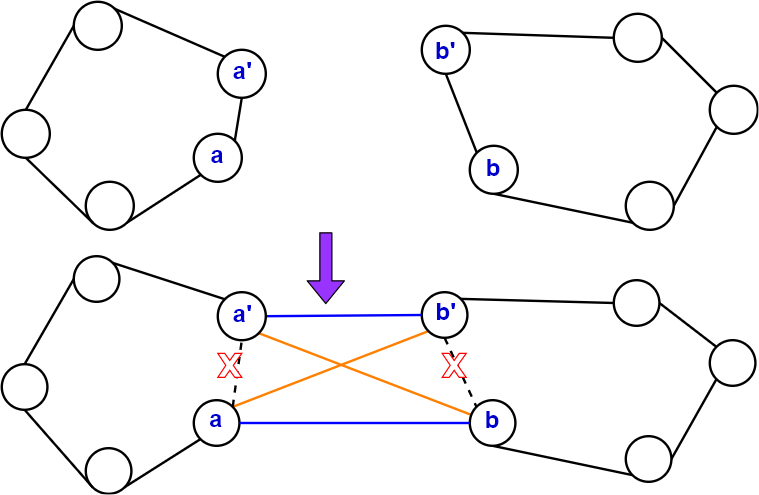
\includegraphics[scale=0.38]{Images/patching}
  \caption{\footnotesize{Esempio di patching}} \label{patching} 
\end{center} 
\end{figure}
Per scegliere quale ramo per ogni componente connessa sia più conveniente eliminare e con quale sia più conveniente sostituirlo, è necessario minimizzare la variazione di costo che quest'operazione comporterebbe, cioè scegliere il minimo tra: \\\\
$min \begin{cases}
\Delta \;(a,b)\;=c_{ab'} + c_{ba'} - c_{aa'} - c_{bb'}\\ 
\Delta' \;(a,b)\;=c_{ab} + c_{b'a'} - c_{aa'} - c_{bb'}\\ 
\end{cases}
\forall \; a,b \in V : comp(a)\neq comp(b)$
\\\\
L'operazione di fusione di due componenti connesse può essere ripetuta finché la soluzione non diventa ammissibile. In questo modo, al termine, è possibile restituire una soluzione accettabile, ma senza garanzia che sia ottima.\\
Nella nostra implementazione è stato scelto di mantenere invariata ad ogni iterazione una delle componenti connesse e di espanderla fondendola a quella più vicina. Grazie a questa scelta viene minimizzato il numero di rami per cui è necessario modificare la struttura dati che li memorizza.\\
Per poter implementare l'algoritmo è necessario utilizzare due diversi tipi di callback messe a disposizione da CPLEX. La prima appartiene alla tipologia delle lazyconstraintcallback  ed è necessaria per ricevere la soluzione trovata dal programma e rielaborarla. A questa soluzione viene applicato l'algoritmo di patching ed il risultato viene memorizzato all'interno in una struttura dati accessibile anche dalla seconda callback dell'utente. Per garantire che la user-callback sia thread-safe, la struttura dati nominata è stata organizzata di  modo tale che ogni thread accedesse ad una sua specifica porzione.\\
La seconda callback necessaria è un heuristic callback e permette all'utente di suggerire a CPLEX una soluzione da cui proseguire la computazione. Questa soluzione sarà quella memorizzata nella struttura dati dalla prima callback e verrà utilizzata dal
programma solo nel caso in cui sia migliore dell'incumbent attuale.\\
Utilizzando, invece, le generic callback non è necessario implementare due diverse user-callback. è sufficiente invocare la callback in due diversi contesti (uno per ricevere la soluzione di cplex, (CPX\_CALLBACKCONTEXT\_CANDIDATE) e l'altro per suggerire il risultato del patching (CPX\_CALLBACKCONTEXT\_LOCAL\_PROGRESS)). I due diversi casi andranno gestiti dall'interno della funzione stessa.\\
Complessivamente il costo di quest'algoritmo è $O(n^2)$, dove $n$ è il numero di nodi.(verificare)\\
\begin{algorithm}[H]
\DontPrintSemicolon
\KwIn {$\mathtt{x}$= soluzione di un problema di TSP con più componenti connesse\newline}
\KwOut {$\mathtt{y}$= soluzione intera formata da un'unica componente connessa}
\BlankLine
$\mathtt{n\_comps \gets} numero componenti connesse della soluzione$\;
\BlankLine
$\mathtt{c_1\gets}\{0,...,0\}$\;
\BlankLine
\While{$n\_comps > 1$}{
\BlankLine
$\mathtt{c_1 \gets first\_subtour(}x\mathtt{)}$\;
\BlankLine
$\mathtt{c_2 \gets nearest\_subtour(}c_1\mathtt{)}$\;
\BlankLine
$\mathtt{merge\_component(}c_1,c_2\mathtt{)}$\;
\BlankLine
$\mathtt{update(}n\_comps\mathtt{)}$\;
}
$\mathtt{y \gets} c_1$\;
\caption{Patching}
\end{algorithm}

\section{Algoritmi Math-Heuristici}
Gli algoritmi euristici sono progettati per risolvere istanze del problema in tempi significativamente più brevi rispetto agli algoritmi esatti. Di conseguenza, però, al termine della computazione non garantiscono di ottenere una soluzione ottima, ma solo una sua buona approssimazione ammissibile. Gli algoritmi Math-euristici sfruttano l'approccio utilizzato dai metodi euristici ma sfruttano la programmazione matematica, introducendo nuovi vincoli al modello. L'algoritmo che maggiormente rappresenta questo metodo è il Soft Fixing (vedi Sezione \ref{soft fixing}). \\
Durante la computazione della soluzione CPLEX utilizza diversi algoritmi euristici e math-euristici e variando alcuni parametri, è possibile variare la frequenza con cui vengono applicati o il tempo a loro dedicato. 

\subsection{Hard Fixing}\label{hard fixing}
Un primo algoritmo math-euristico di semplice implementazione è l'Hard-fixing, composto dalle seguenti fasi:
\begin{enumerate}
\item{Impostazione di un time limit per la computazione di una soluzione;}
\item{Calcolo della soluzione;}
\item{Selezione, in maniera randomica, di un sottoinsieme di rami appartenenti alla soluzione ottima (Figura \ref{selezione_rami}). 
Il numero di questi è definito da una percentuale fissata sul totale dei lati scelti. Le variabili dei rami selezionati, sono impostate al valore $1$;}
\end{enumerate}
\begin{figure}[h] 
\begin{center} 
  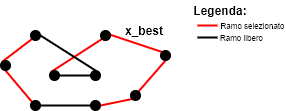
\includegraphics[scale=0.38]{Images/x_best} 
  \caption{\footnotesize{Selezione rami}}
  \label{selezione_rami} 
\end{center} 
\end{figure}
Questi passaggi vengono eseguiti in maniera ciclica per un numero fissato di iterazioni. In questo modo, ad ogni computazione della soluzione, CPLEX dovrà risolvere un problema più semplice di quello originale, essendo molte variabile del modello già selezionate nella \textbf{Fase 3} dell'iterazione precedente.\\
All'interno del programma sviluppato, il time limit nominato nella \textbf{Fase 1} è dato da una frazione della deadline complessiva inserita dall'utente e dipende dal di diverse percentuali che si desidera utilizzare. All'ultima iterazione il time limit viene ricalcolato in base al tempo rimanente al programma, rispetto alla deadline complessiva inserita dall'utente. Ad ogni computazione il costo la soluzione potrà solo migliorare o restare invariato rispetto alla precedente soluzione calcolata.\\
La percentuale relativa al numero di rami da fissare può variare ad ogni iterazione. Generalmente viene utilizzata una percentuale alta nelle prime iterazioni, in cui la soluzione non è ancora stata raffinata, e viene ridotta nelle successive iterazioni, in modo da aumentare i gradi di libertà nella computazione della soluzione per CPLEX.\\
La selezione in maniera randomica degli archi nella \textbf{Fase 3}, garantisce che l'algoritmo termini poichè non vengano fissate sempre le stesse variabili. 
% LEGGILA
Particolare attenzione deve essere posta al fatto di lasciare nell'insieme dei rami scelti randomicamente solo quelli selezionate all'iterazione immediatamente precedente. Nell'implementazione sviluppata, le percentuali utilizzate sono state memorizzate in un vettore in questo ordine $\lbrace$ 90, 75, 50, 25, 10, 0 $\rbrace$.
Di seguito viene inoltre riportato lo pseudocodice dell'implementazione sviluppata:\\\\
\begin{algorithm}[H]
\DontPrintSemicolon
\KwIn {$\mathtt{model}$= modello TSP simmetrico senza vincoli di Subtour Elimination \newline
$\mathtt{deadline}$= time limit complessivo dell'algoritmo\newline
$\mathtt{percentage}$= array con i valori delle percentuali di fissagio degli archi\newline
$\mathtt{num_nodi}$= numero di nodi dell'istanza tsp\newline}
\KwOut {$\mathtt{x}$= soluzione intera senza subtour}
\BlankLine
$\mathtt{n \gets}0$\;
\BlankLine
\While{$expired\_time < deadline$}{
 \BlankLine\BlankLine
 $\mathtt{setTimeLimit()}$\;
 $\mathtt{x \gets solve(}model\mathtt{)}$\;
 \BlankLine\BlankLine
 \For{$\mathtt{j \gets}0$ \KwTo $num\_nodi-1$}{
   $k \gets random(0,1)$\;
   \BlankLine\BlankLine
   \If{$  100*k \leq percentage[n\;mod\;leght(percentage)]  $}{
     \BlankLine
     $Aggiungi \;\;\mathtt{x\_best[j]}\;\;to\;\;S\;where\;S=\{edges\;to\;fix\}$
   }
   \BlankLine
}
\BlankLine
\ForAll{$x_{i,j} \in S$}{
$\mathtt{x_{i,j} \gets}1$\;
\BlankLine
}
\BlankLine
$\mathtt{n \gets}n+1$\;
\BlankLine
}
\caption{Hard Fixing}
\end{algorithm}

\subsection{Soft Fixing}\label{soft fixing} %controlla che siano local branching
Il metodo seguente fa utilizzo di vincoli aggiuntivi, detti di \textbf{Local Branching}. L'approccio utilizzato è simile a quello dell'Hard Fixing, ma la scelta delle variabili da imporre a 1 non viene fatta in maniera randomica ma viene lasciata a CPLEX.\\
Partendo da una soluzione intera ammissibile del TSP $x^H$, viene aggiunto un vincolo sulle variabili con valore $1$ in $x^H$:\\
$$\underset{e\in E\; : \; {x_e}^{H}=1}\sum{x_e}\;\geq\; 0.9\;n$$
dove la sommatoria indica il numero di variabili, uguali a $1$ in $x^H$, che non cambieranno il loro valore e \textbf{n} indica il numero di archi selezionati, pari al numero di nodi.\\
In questo caso, il vincolo permetterà a CPLEX di fissare il 90\% dei rami scelti in $x^H$ e avere il 10\% di libertà.
Un modo alternativo di scrivere lo stesso vincolo è il seguente:
$$\underset{e\in E\; : \; {x_e}^{H}=1}\sum{x_e}\;\geq\; n-k$$
dove k=2,...,20 e rappresenta i gradi di libertà di CPLEX nel calcolare la nuova soluzione.\\
Ad ogni iterazione viene aggiunto un nuovo vincolo di local branching, basato sull'attuale soluzione restituita da CPLEX, e viene rimosso il vincolo aggiunto nell'iterazione precedente.\\
Non scegliendo in maniera randomico i lati da selezionare, come invece accade nell'Hard Fixing, se non dovesse esserci alcun miglioramento del costo e quindi cambiamento della soluzione, i lati selezionati da CPLEX con il nuovo \textbf{local branching}, sarebbero gli stessi dell'iterazione precedente. Per ovviare tale problema, il valore di k viene inizializzata a 2 e, nel caso in cui non dovesse migliorare la soluzione, viene incrementata.\\
Da dati sperimentali, si è appurato come questo metodo aiuti CPLEX a convergere più velocemente alla soluzione ottima e che valori di k superiori a 20 non aiutino a raggiungere risultati migliori.\\
L'aggiunta di un local-branching permette di analizzare in maniera più semplice e veloce lo spazio delle soluzioni. Normalmente per farlo, dovrebbere essere enumerati gli elementi di questo spazio ma ciò comporterebbe la creazione di un numero molto elevato di possibli soluzioni per via della NP-difficoltà del TSP.\\
Definita una soluzione intera ammissibile $x^H$ e utilizzando la distanza di Hamming, le soluzioni $k-opt$, rispetto ad $x^H$, sono quelle che hanno distanza k da $x^H$ (vedi Figura \ref{opt}).\\
\begin{figure}[h] 
\begin{center} 
  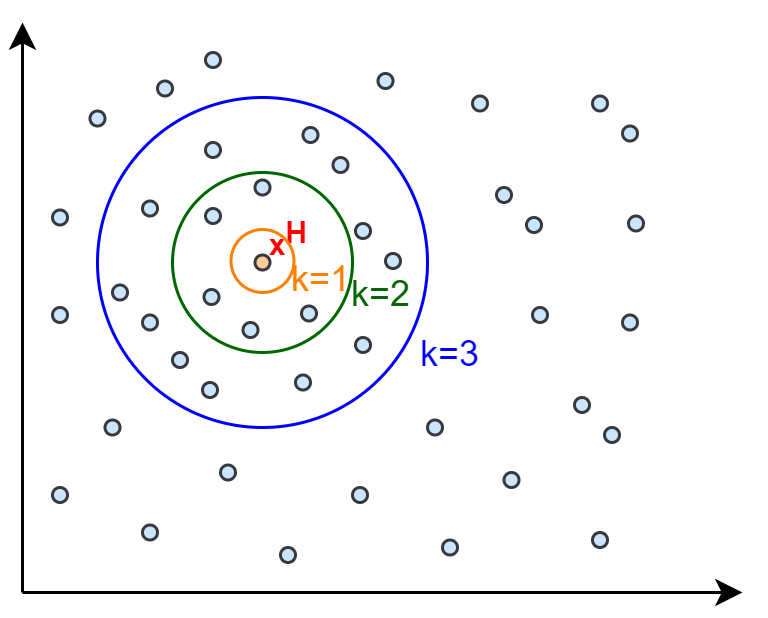
\includegraphics[scale=0.38]{Images/opt}
  \caption{\footnotesize{Spazio delle soluzioni e distanza di Hamming.}} \label{opt} 
\end{center} 
\end{figure}
Se, invece del local branching, venisse utilizzata l'enumerazione delle soluzioni, dovrebbero essere generate per \textbf{k} generico circa $n^k$ soluzioni a distanza k da $x^H$. In seguito dovrebbero essere analizzate tutte per individuare quella con costo minore di $x^H$.\\
L'utilizzo del local branching può essere adottato con anche problemi generici e non solo con TSP. Di seguito viene riportato l'aprroccio da seguire per generare tutte le soluzioni a distanza minore o uguale di R dalla soluzione euristica di partenza $x_H$:
\begin{align}
& min \{ c^T x:\;\;Ax=b,\;x\in\{0,1\}^n\} \\ \notag \\
& \underset{j\in E:{x_j}^H=0}\sum{x_j}\;+ \underset{j\in E:{x_j}^H=1}\sum{1-x_j}=\; \leq R
\end{align}
dove \textbf{(3.15)} rappresenta la distanza di Hamming dalla nuova soluzione computata $x$ da $x_H$. L'obiettivo del Soft-fixing è cercare di migliorare il costo della soluzione, guardando quelle più vicine possibili a quella attuale. Nella \textbf{Figura \ref{local_exe}} viene riportato un esempio di una possibile evoluzione dell'algoritmo nella ricerca dell'ottimo, evindenziandone le soluzioni trovate di volta in volta.
\begin{figure}[h] 
\begin{center} 
  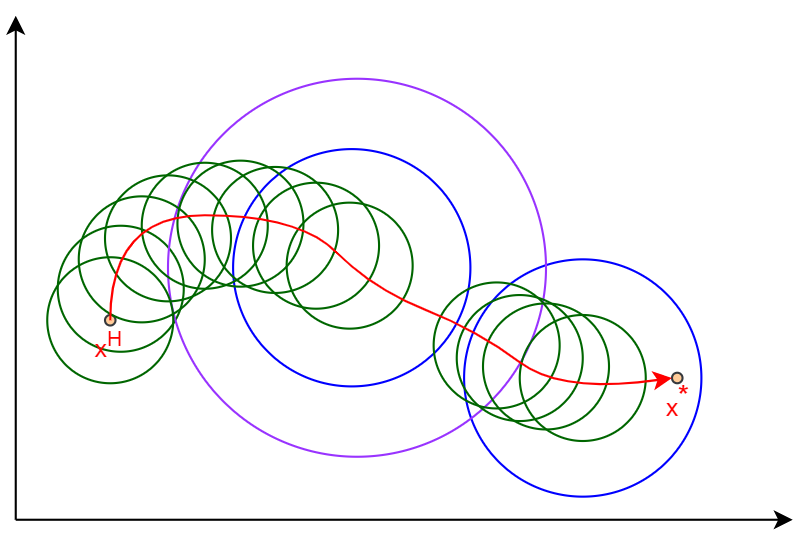
\includegraphics[scale=0.38]{Images/local_exe}
  \caption{\footnotesize{Esempio di esecuzione dell'algoritmo nello spazio delle soluzioni.}} \label{local_exe} 
\end{center} 
\end{figure}
\chapter{Algoritmi euristici}\label{HEURISTIC}
In questo capitolo verranno trattati algoritmi euristici che non fanno uso di CPLEX. La necessità di non utilizzare CPLEX si ha per istanze con un elevato numero di nodi per cui la risoluzione del tableau diventerebbe un'operazione molto onerosa per via dell'alto numero di variabili coinvolte.\\
Attraverso gli algoritmi euristici, viene computata un'approssimazione della soluzione ottima che spesso può essere anche sfruttata inizialmente dal risolutore CPLEX, per aiutarlo nello risoluzione di problemi anche più complessi.\\
Ad esempio può essere aggiunta prima della computazione, utilizzando la funzione \textit{CPXaddmipstarts()}, o, se già definita, può essere modificata tramite \textit{CPXchgmipstarts()}.\\
Per progettare un efficiente algoritmo euristico, questo deve essere composto da due fasi che si alternino:
\begin{itemize}
\item{\textbf{Intensificazione o raffinamento}\\
In questa fase la soluzione corrente viene migliorata fino al raggiungimento di un ottimo (locale o globale) nello spazio delle soluzioni.
}
\item{\textbf{Diversificazione}\\
Fase in cui la soluzione viene perturbata con una politica predefinita affinché si allontani da un ottimo locale nello spazio delle soluzioni.
}
\end{itemize}


\section{Algoritmi di costruzione}\label{construction_alg}
Questa tipologia di algoritmi euristici è fondamentale per la computazione di una prima soluzione ammissibile del problema.
\subsection{Nearest Neighborhood}
L'algoritmo Nearest Neighborhood è basato su un approccio di tipo greedy. Inizialmente viene selezionato un nodo generico tra quelli che compongono il grafo ed in seguito vengono aggiunti iterativamente degli archi del grafo, secondo il criterio enunciato nella seguente sezione.\\
In ciascuna iterazione vengono analizzati gli archi uscenti dal nodo selezionato all'iterazione precedente e viene selezionato tra questi il ramo collegato all'estremo più vicino. Il nuovo nodo raggiunto verrà impostato come punto di partenza nell'analisi dei costi dell'iterazione successiva (vedi Figura \ref{nearest_neighborhood}).
All'ultima iterazione viene selezionato invece l'arco che collega l'ultimo nodo visitato al nodo scelto randomicamente all'inizio dell'algoritmo.\\
Il problema di questo algoritmo è che in ogni iterazione viene selezionato esclusivamente il vertice più vicino a quello scelto precedentemente, senza però cercare di prevedere e migliorare la futura evoluzione del costo del tour, creato dall'algoritmo.\\
Come in Figura \ref{nearest_neighborhood}, la scelta dell'arco di costo minimo non implica che in seguito venga generata la soluzione ottima. La scelta del nodo iniziale è fondamentale in quanto una perturbazione della partenza genera un tour differente.\\
Definito \textbf{n} come il numero di nodi presenti nel grafo, si avranno quindi n soluzioni differenti, ottenute ciascuna attraverso l'applicazione dell'algoritmo partendo da una diversa scelta iniziale.\\
\begin{figure}[H] 
\begin{center} 
  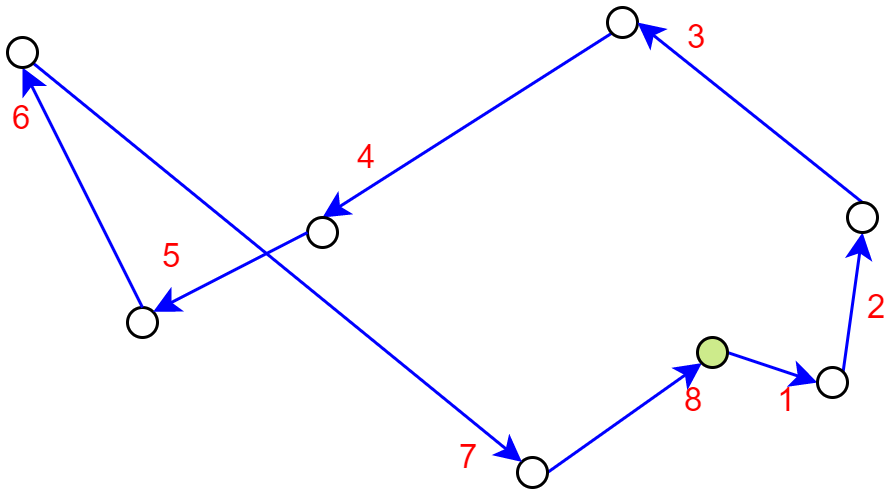
\includegraphics[scale=0.3]{Images/nearest_neighborhood}\\ 
  \caption{\footnotesize{Esempio di esecuzione di Nearest Neighborhood.}}
  \label{nearest_neighborhood} 
\end{center} 
\end{figure}

\subsection{Heuristic Insertion}
L'algoritmo seguente usa un approccio simile al precedente ma prevede inizialmente la selezione di un ciclo, a cui verranno apportate modifiche per ottenere una soluzione iniziale ammissibile del problema. Per definire il ciclo di partenza vengono utilizzati diversi metodi. Di seguito sono riportati i due più utilizzati:
\begin{itemize}
\item{\textbf{Selezione di due nodi}\\
Vengono scelti i due nodi più lontani tra loro nel grafo, o due nodi casuali, e vengono collegati mediante i due archi orientati, che li connettono tra loro.
}
\item{\textbf{Inizializzazione geometrica}\\
Nel caso in cui i nodi del grafo appartengano ad uno spazio bidimensionale, ne viene calcolata la convex-hull e questa viene utilizzata come ciclo di partenza.
}
\end{itemize}
Questa prima soluzione viene modificata iterativamente e per ogni coppia di nodi non appartenenti al ciclo \textbf{C}, restituito dall'iterazione precedente, viene calcolato l'extramileage $\Delta_h$ come segue:
$$\Delta_h = \underset{(a,b)\in C}{min} (c_{ah}+c_{hb}-c_{ab})$$
con $c_{ij}=$ costo dell'arco che collega i a j (vedi Figura \ref{partial_cycle}).\\
Alla fine di ciascuna iterazione viene aggiunto nel grafo il nodo \textbf{k} che minimizza l'\textbf{extra-mileage} (vedi Figura \ref{insertion}):\\
$$k = arg\underset{h}{min}\;\Delta_{h}$$
\begin{figure}[H] 
\begin{center} 
  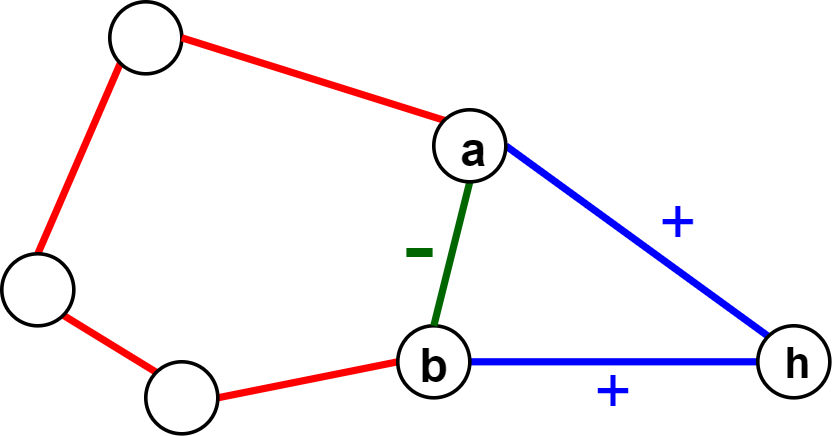
\includegraphics[scale=0.2]{Images/partial_cycle}\\ 
  \caption{\footnotesize{Parte del calcolo dell'extramileage del nodo \textbf{h}.}}
  \label{partial_cycle}
\end{center}
\end{figure}
\vspace{2 cm}
\begin{figure}[h] 
\begin{center} 
  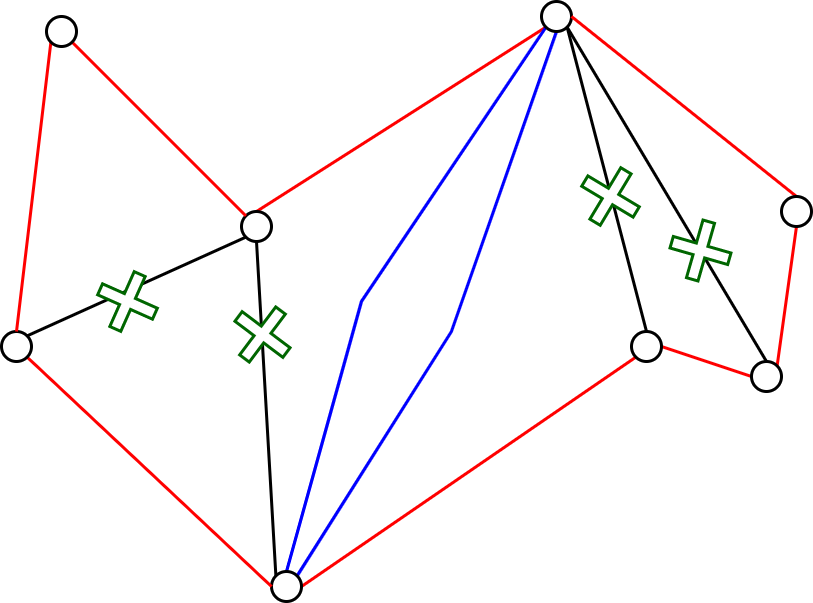
\includegraphics[scale=0.3]{Images/insertion}\\ 
  \caption{\footnotesize{Esempio dell'applicatione di Heuristic insertion.}}
  \label{insertion}
\end{center}
\end{figure}

\subsection{GRASP}
Il metodo Greedy Randomized Adaptive Search Procedure (GRASP) è un approccio algoritmico che permette di aggiungere una componente aleatoria alla computazione deterministica del minimo di un insieme di valori.\\
Ad ogni iterazione dei due precedenti algoritmi di costruzione, invece di selezionare l'arco di costo minimo o l'extra-mileage minimo, vengono memorizzati i rami di costo minore e le scelte con extra-mileage minore.\\
Tra le possibili mosse salvate, ne viene scelta randomicamente una. Nel programma sviluppato, oltre ai precedenti algoritmi di costruzione, ne sono state implementate anche delle varianti che fanno uso del GRASP. In questo caso sono state memorizzate le tre scelte migliori in ogni iterazione.\\
Tali varianti permettono di modificare in maniera aleatoria l'evoluzione del tour, in modo da evitare che, nelle ultime iterazioni dell'algoritmo, le scelte possibili siano legate esclusivamente ad elevati incrementi della funzione obiettivo.\\
Ciò evita ad esempio che nel Nearest Neighborhood possano esserci numerose scelte come l'ultima effettuata in Figura \ref{nearest_neighborhood}.\\
Nella Sezione \ref{construction_perf}, vengono confrontati tramite performance profile, gli algoritmi precedentemente nominati.

\section{Algoritmi di raffinamento}
Una volta ottenuta una prima soluzione è necessario migliorarla per avvicinarsi il più possibile all'ottimo. Gli algoritmi utilizzati con questo scopo sono detti \textit{algoritmi di raffinamento}. Nel capitolo precedente sono già stati descritti due procedimenti di questo tipo, l'Hard Fixing e il Soft Fixing (vedi sottosezioni \ref{hard fixing} e \ref{soft_fixing}). In questa sezione verranno invece analizzati algoritmi di raffinamento che non utilizzino funzioni messe a disposizione da CPLEX.

\subsection{Algoritmo di 2-ottimalità}
Nelle soluzioni restituite dagli algoritmi euristici di costruzione sono spesso presenti incroci tra coppie di rami. La loro presenza implica che la soluzione non è ottima, in quanto per le proprietà dei triangoli esisterà sempre una tour che eviti l'incrocio e che sia di costo minore. Infatti, in riferimento alla Figura \ref{cross},
\begin{equation}
\begin{cases}
ad < \alpha \;+\; \delta \\ \notag
cb < \gamma \;+\; \beta
\end{cases} 
\Rightarrow
\;\;ad+cb<\alpha + \delta +\gamma + \beta
\end{equation}. 
\begin{figure}[H] 
\begin{center} 
  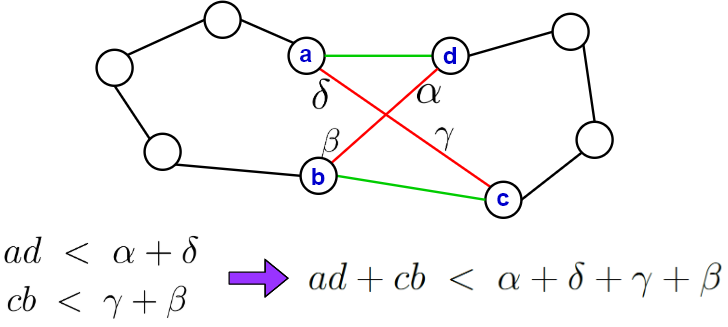
\includegraphics[scale=0.5]{Images/triangle_property}
  \caption{\footnotesize{Non ottimalità di una soluzione con incroci.}}
  \label{cross}
\end{center}
\end{figure}
L'algoritmo di 2-ottimilità prende il nome dalla modalità utilizzata iterativamente per modificare la soluzione ricevuta in ingresso. In ogni iterazione viene individuato un incrocio tra due rami, appartenenti al tour. Gli estremi di tali archi vengono collegati in maniera differente. Complessivamente per ogni incrocio, viene effettuato uno scambio tra coppie di rami (2-opt move) in modo da ridurre ulteriormente il costo della soluzione restituita.\\
Nell'implementare tale algoritmo non è necessario individuare ciascun incrocio della soluzione di partenza ma è sufficiente analizzare tutte le coppie di rami presenti e verificare se, scambiandole con un'altra coppia ammissibile, si verifichi un miglioramento della funzione obiettivo.
\begin{figure}[H] 
\begin{center} 
  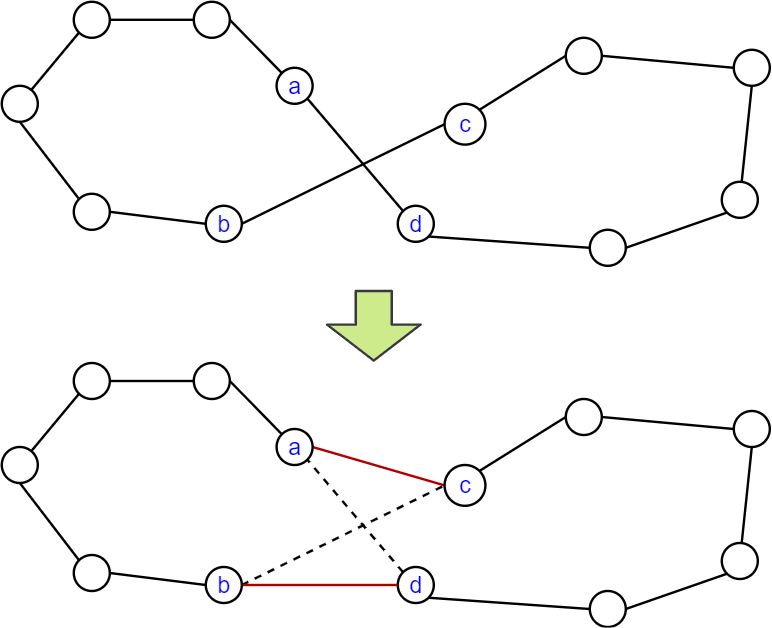
\includegraphics[scale=0.35]{Images/swap}\\ 
  \caption{\footnotesize{Esempio di eliminazione di un incrocio.}}
  \label{swap}
\end{center}
\end{figure}
Riferendosi alla Figura \ref{swap}, un possibile miglioramento viene calcolato come segue:\\
$$\Delta = (c_{ac} + c_{bd}) - (c_{ad} + c_{bc})$$
e solo nel caso in cui $\Delta$ sia negativo, la sostituzione viene effettuata.\\
Applicando una 2-opt move al circuito attuale, viene generato un tour appartenente all'intorno di 2-ottimalità della precedente soluzione. Ripetendo iterativamente tale procedimento si raggiunge un ottimo locale, in cui non esistono più possibili miglioramenti della funzione obiettivo. Questo processo è rappresentato in Figura \ref{two_optimality}. 
\begin{figure}[H] 
\begin{center} 
  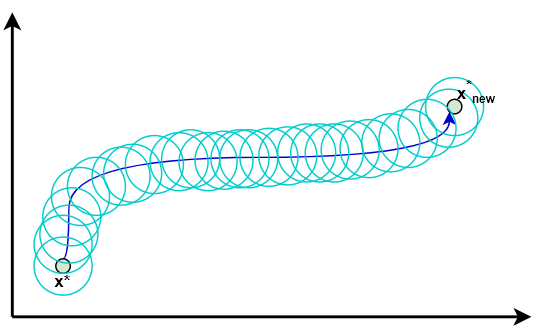
\includegraphics[scale=0.3]{Images/two_optimality}\\ 
  \caption{\footnotesize{Aggiornamento della soluzione nell'intorno di 2 ottimalità.}}
  \label{two_optimality}
\end{center}
\end{figure}
Poichè il calcolo del $\Delta$ avviene in tempo costante e deve essere svolto per ogni coppia di rami, il tempo complessivo per la computazione è $O(n^2)$, con $n$ pari al numero di nodi dell'istanza.\\
Un procedimento analogo a tale algoritmo viene utilizzato anche nel Soft Fixing, in cui però la dimensione dell'intorno in cui cercare la nuova soluzione varia (vedi Figura \ref{local_exe}).\\
Nel programma sviluppato, è stata utilizzata questo tecnica per rimuovere gli incroci all'interno di un tour.
 
\subsection{Algoritmo di 3 ottimalità}
L'algoritmo di 3 ottimalità è analogo a quello analizzato nella sezione precedente, ma considera intorni di grandezza maggiore. In questo caso, quindi, due soluzioni nell'intorno differiscono per 3 rami. In Figura \ref{three_optimality} viene riportata la rappresentazione delle possibili 3-opt move.\\
\begin{figure}[H] 
\begin{center} 
  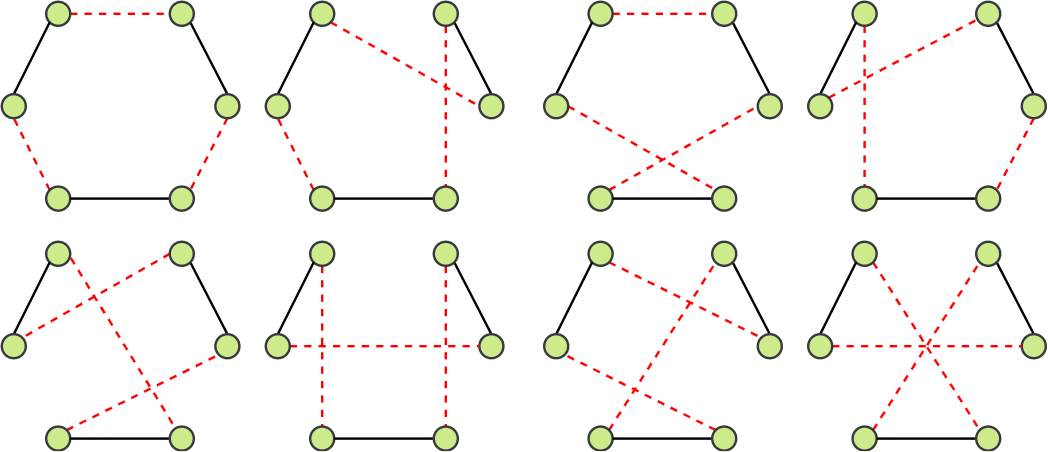
\includegraphics[scale=0.35]{Images/3_swap}
  \caption{\footnotesize{Tutte le possibili combinazioni di scambi di 3 ottimalità.}}
  \label{three_optimality}
\end{center}
\end{figure}
L'algoritmo impiega in tutto $O(n^3)$ (con $n$ numero di nodi) per trovare un ottimo locale, essendo $O(n^3)$ il numero di terne di rami esistenti e poiché il numero di possibili scambi di 3 ottimalità è costante. Su istanze con un elevato numero di nodi, il tempo di calcolo risulterebbe essere troppo lungo per riuscire a computare una soluzione. All'interno del programma sviluppato, non è stata implementato tale algoritmo.

\section{Meta-euristici}
Gli algoritmi di raffinamento appena visti si occupano di migliorare il più possibile una soluzione già calcolata, attraverso meccanismi di local search. In questo modo, dopo un determinato numero di iterazioni, viene raggiunto un nuovo ottimo locale.\\
Gli algoritmi descritti in questa sezione perturbano la soluzione allontanandola dall'attuale ottimo locale e cercando di avvicinarsi il più possibile all'ottimo globale.\\
Questi metodi rappresentano approcci più generali di quelli descritti precedentemente e sono applicabili anche a problemi differenti rispetto al TSP. Tali tecniche infatti permettono essenzialmente di esplorare lo spazio delle soluzioni, evitando di stazionare in minimi o massimi locali con valori della funzione obiettivo molto lontani dall'ottimo globale.

\subsection{Multi-start}
Un primo e intuitivo approccio per allontanarsi da un ottimo locale è quello descritto dalla politica multi-start. Questa consiste nel definire diverse soluzioni attraverso un algoritmo di costruzione tra quelli descritti, ad esempio, nella Sezione \ref{construction_alg}.\\
A ciascuna di esse viene poi applicato un algoritmo di raffinamento ed in seguito  viene scelta solo la soluzione con costo minore tra quelle generate. In questo modo vengono analizzati diversi ottimi locali nello spazio delle soluzioni (vedi Figura \ref{multi_start}). 
\begin{figure}[H] 
\begin{center} 
  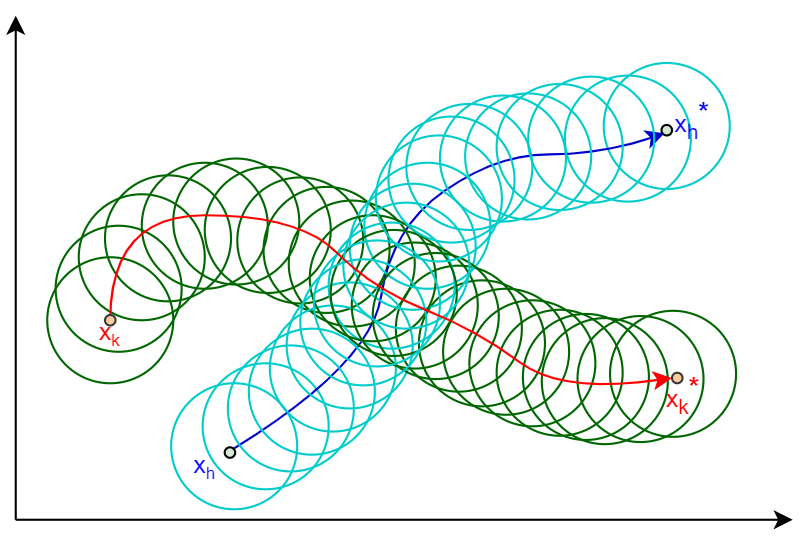
\includegraphics[scale=0.4]{Images/multistart}\\ 
  \caption{\footnotesize{Due possibile esecuzioni di un algoritmo di raffinamento con partenze da due soluzioni diverse.}}
  \label{multi_start}
\end{center}
\end{figure}
Un lato negativo di tale approccio consiste nel fatto che ogni volta che viene generata una nuova soluzione del problema, vengono perse le informazioni relative ai tour generati in precedenza. La soluzione implementata all'interno del programma è basata sul multithreading. Infatti viene generato un numero di soluzioni pari al numero di thread specificati.\\
Ciascun thread genera parallelamente agli altri una nuova soluzione e solo al termine della computazione, la confronta con la migliore. Nel caso in cui il costo della soluzione trovata sia inferiore a questa, la aggiorna. \\
Nella Sezione \ref{construction_perf} viene analizzato il costo ottenuto dalla nostra implementazione, utilizzando 12 thread e modificando l'algoritmo di costruzione utilizzato.\\

\subsection{Variable Neighborhood Search}
Il Variable Neighborhood Search (VNS) è un algoritmo che cerca di migliorare l'ottimo locale attuale, ricevuto in input, analizzando intorni di ottimalità di grandezza differente.\\
Nel caso in cui non si trovi una nuova soluzione, di costo migliore di quella attuale nei vari intorni di grandezza k, l'algoritmo prevede che venga scelto un certo numero di rami in maniera randomica da sostituire con altri lati\cite{VNS_CITE}. In questo modo si impone un aggiornamento peggiorativo in termini di costo, nella speranza che nel nuovo intorno selezionato sia possibile trovare una soluzione che si allontani dall'ottimo locale di partenza (vedi Figura \ref{VNS_img}).\\
 \begin{figure}[H] 
\begin{center} 
  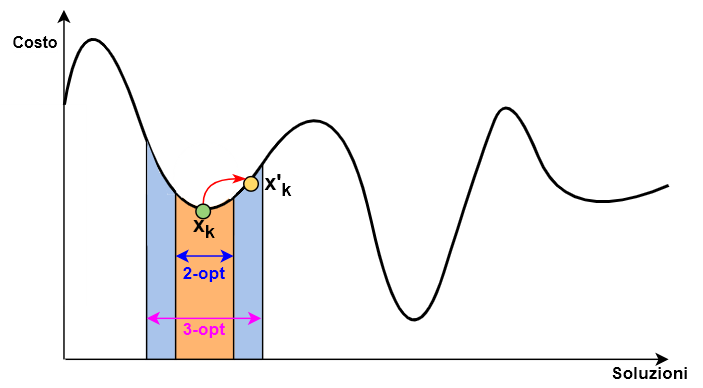
\includegraphics[scale=0.4]{Images/VNS}\\ 
  \caption{\footnotesize{Esempio di analisi dello spazio delle soluzioni fatto dal VNS.}}
  \label{VNS_img}
\end{center}
\end{figure}
L'algoritmo termina allo scadere di una deadline, inserita dall'utente, o dopo un determinato numero di iterazioni, restituendo la miglior soluzione trovata fino a quell'istante. Utilizzando questo approccio gran parte della soluzione di partenza viene conservata evitando di perdere le informazioni elaborate precedentemente eseguendo l'algoritmo.\\
La nostra implementazione dell'algoritmo VNS non è però quella classica ma una variante detta VNS ibrido\cite{hybrid_VNS}. Nell'Algoritmo \ref{VNS} viene descritto lo pseudo-codice di tale metodo.\\
Partendo dalla sequenza di visita dei nodi nella soluzione locale, passata in ingresso all'algoritmo, la procedura analizza tutti i tour ottenuti invertendo due nodi a distanza k nella sequenza, con $k=1,...,n/2$. Se viene individuata una soluzione con costo inferiore, allora questa viene considerata come il nuovo ottimo locale. Invece se non dovesse esistere alcuno scambio migliorativo, viene scelta in maniera randomica una nuova soluzione dall'insieme:
$$\biggl\{\{y\}\cup \bigcup_{k=1}^{\lceil n/2 \rceil}{N_k(y)}\biggr\}$$
con probabilità pari a:
$$p=\frac{costo^{-1}(x)}{\underset{z \in {\bigcup_{k=1}^{\lceil n/2 \rceil}{N_k(y)}}}\sum{costo^{-1}(z)}}$$
Nell'implementazione sono state sviluppate due versioni di questo algoritmo, in base alle probabilità utilizzate nel selezionare due nodi da scambiare: 
\begin{itemize}
\item{\textbf{Hybrid VNS}\\
questa prima soluzione segue la procedura precedentemente descritta e seleziona una nuova sequenza dall'insieme $\{{y}\cup \bigcup_{k=1}^{\lceil n/2 \rceil}{N_k(y)}\}$ e poi vi applica un algoritmo di raffinamento.} 
\item{\textbf{Hybrid VNS Uniform}\\
questa variante invece seleziona due nodi della sequenza di visita, secondo una probabilità uniforme, e li scambia. La sequenza risultante, dopo essere stata migliorata mediante un algoritmo di raffinamento, viene utilizzata come nuovo minimo locale.}
\end{itemize}
\begin{algorithm}[h]
\DontPrintSemicolon
\KwIn {$\mathtt{x =\{x_1,x_2,...,x_n\}}$= sequenza di visita dei nodi nella soluzione di partenza (ottimo locale)\newline}
\KwOut {$\mathtt{x}$= soluzione migliore aggiornata dall'algoritmo}
\BlankLine
\While{$'deadline\;not\;expired'$ $\wedge$ $count<MAX\_COUNT$}{
\BlankLine
$\mathtt{y\gets} x$\;
$\mathtt{k\gets}1$\;
\BlankLine
 \While{$k\leq \lceil n/2 \rceil$}{
  \BlankLine
  $N_k(y) = \{ (y_1,...,y_{(i+k)mod\;n},...,y_i, ..., y_n)\; :\; 1\leq i\leq n\}$\;
  \BlankLine
  \If{$\underset{z\in N_k(y)}{min}\{cost(z)\}<cost(x)$}{
	 $\mathtt{x\gets} \underset{z\in N_k(y)}{argmin(cost(z))}$\;
     $\mathtt{y\gets} \underset{z\in N_k(y)}{argmin(cost(z))}$\;
	 $\mathtt{break}$\;
     \BlankLine
  }
  \BlankLine
  $\mathtt{k}\gets k+1$\;
  \BlankLine
 }
 \If{$k>\lceil n/2 \rceil$}{
    \BlankLine
    $\mathtt{y}\gets \mathtt{new\_random\_sol(} y \mathtt{)}$\;
    \BlankLine
 }
  $\mathtt{count}\gets count+1$\;
}
 \caption{VNS ibrido}\label{VNS}
\end{algorithm}
\subsection{Tabu Search}
Il metodo Tabu Search fu ideato da Fred W. Glover. Dato un ottimo locale, l'idea di Glover permette di modificare la soluzione corrispondente anche peggiorandone il costo, con l'obiettivo di esplorare maggiormente lo spazio delle soluzioni. Ad ogni iterazione dell'algoritmo la soluzione viene modificata con un nuovo tour, appartenente al suo intorno di 2-ottimalità.\\
Per evitare che queste modifiche portino ad esplorare minimi locali già visitati, viene creata una lista di "mosse vietate", detta \textit{Tabu List}. In questo modo il costo del tour attuale viene aumentato per un certo numero di iterazioni, finché le uniche modifiche ammissibili della soluzione corrente permettano solo di migliorare il valore della funzione obiettivo. Questa fase rappresenta la diversificazione della soluzione.\\
In seguito viene effettuata una fase di intensificazione, mediante l'applicazione dell'algoritmo di 2-ottimalità, fino al raggiungimento di un nuovo minimo locale.\\
Nella nostra implementazione la lista viene riempita con i rami che vengono rimossi dal tour attuale per creare la nuova soluzione.\\
Aumentando costantemente di dimensione la lista Tabu si rischia, ad un certo punto, che non sia più possibile modificare il tour presente. Per evitare ciò generalmente viene scelta una capienza massima della lista, detta \textit{tenure}. Una volta riempita la Tabu List i rami vengono aggiunti rispettando la politica FIFO (First In First Out).\\
Per aumentare le prestazioni dell'algoritmo è possibile far variare le dimensioni della Tabu List tra due valori. Nella fase di diversificazione le dimensioni della lista aumentano fino ad una soglia massima, mentre durante l'intensificazione la tenure diminuisce fino ad un valore minimo fissato, per lasciare maggiore libertà all'algoritmo di 2-ottimalità. Nella nostra implementazione la tenure massima ha valore pari ad 1/5 del numero di nodi dell'istanza da risolvere, mentre quella minima è pari alla metà di quest'ultima (vedi Figura \ref{tenure}). Questa variante dell'algoritmo, implementata anche nel nostro programma, in letteratura è conosciuta con il nome di \textit{Reactive Tabu Search}.
 \begin{figure}[H] 
\begin{center} 
  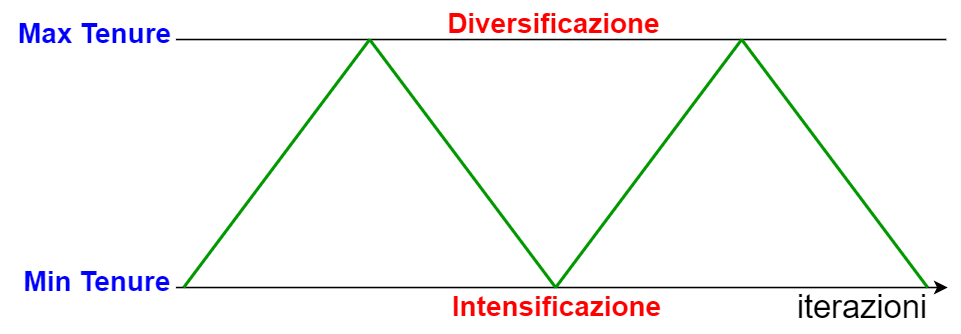
\includegraphics[scale=0.35]{Images/tenure}\\ 
  \caption{\footnotesize{Variazione della tenure.}}
  \label{tenure}
\end{center}
\end{figure}
Come per l'algoritmo precedente, il criterio di terminazione è dato dallo scadere del tempo a disposizione o dal raggiungimento di un numero massimo di iterazioni. La soluzione restituita dall'algoritmo è la migliore individuata fino a quell'istante.\\\\
\begin{algorithm}[H]
\DontPrintSemicolon
\KwIn{$\mathtt{x}$= soluzione di un'istanza di TSP corrispondente ad un ottimo locale\newline
$\mathtt{tenure}$= dimensione massima della Tabu List\newline
$\mathtt{deadline}$= time limit complessivo dell'algoritmo\newline
$\mathtt{num\_iterations}$= numero massimo di iterazioni\newline
$\mathtt{num\_nodi}$= numero di nodi dell'istanza tsp\newline}
\KwOut {$\mathtt{y}$= miglior soluzione trovata}
\BlankLine
$\mathtt{n}=0$\;
\BlankLine
\While{$n < num\_iterations \wedge\;\;'deadline\;not\;expired'$}{
 \BlankLine
 $\mathtt{x' \gets move\_random\_2opt(}x)$\;
 \BlankLine
 \BlankLine
\While{$(check\_tabu\_list(x') ==\;'valid\;move')$}{
  \BlankLine
  $\mathtt{x' \gets move\_random\_2opt(}x\mathtt{)}$\;
}
  $\mathtt{x} \gets x'$\;
  $\mathtt{add\_tabu\_list(}edges\_removed, tenure\mathtt{)}$\;
  \BlankLine
  \If{$cost(x') < cost(x)$}{
    \BlankLine
    $\mathtt{x \gets greedy\_refinement(}x, tabu\_list\mathtt{)}$\;
    \BlankLine  
  }
  \BlankLine
  $\mathtt{n \gets}n+1$\;
}
 \BlankLine
$\mathtt{y}= best\_solution()$\;
\caption{Tabu Search}
\end{algorithm}
\subsection{Simulated Annealing}
L'algoritmo Simulated Annealing si ispira al processo di temperamento dei metalli, in cui un materiale viene raffreddato molto lentamente e in maniera controllata, affinché raggiunga la configurazione di minima energia\cite{SA}. Analogamente, nell'algoritmo viene scelta una funzione, generalmente esponenziale, che simuli la variazione della "temperatura" $T$.\\
Nel corso delle iterazioni, la soluzione corrente può essere aggiornata con un'altra qualsiasi nel suo intorno di 2 ottimalità (Figura \ref{simulated_annealing}). La probabilità di accettare un nuovo tour peggiorativo è una funzione $f(\Delta costo, T)$ che dipende dalla differenza, tra il costo della soluzione attuale e quello della nuova candidata, e dal valore corrente della temperatura. Nel caso in cui avvenga un aumento del costo complessivo della soluzione, la temperatura viene decrementata. In questo modo si riduce la probabilità di accettare un aggiornamento peggiorativo durante l'iterazione successiva. \\
 \begin{figure}[H]
\begin{center} 
  \includegraphics[scale=0.38]{Images/simulated_anneling}
  \caption{\footnotesize{Esempio di esecuzione dell'algoritmo Simulated Annealing.}}
  \label{simulated_annealing}
\end{center}
\end{figure}
Per variare la temperatura, è stata utilizzata la seguente formula \cite{SA}:
$$T = \alpha^{i}\:T\_max \;+\; T\_min$$
dove \textit{T\_max} è la massima temperatura iniziale, \textit{T\_min} è la minima temperatura che può essere raggiunta, \textit{i} è il numero di iterazioni eseguite fino a quel momento e \textit{$\alpha$} è un parametro scelto all'inizio dell'esecuzione. Nello sviluppare questo procedimento sono stati utilizzati i seguenti valori:
\begin{itemize}
\begin{multicols}{3}
\item{\textit{T\_max} = 5000}
\item{\textit{T\_min} = 100}
\item{\textit{$\alpha$} = 0.99}
\end{multicols}
\end{itemize}
Una volta raggiunta la temperatura minima, nel caso in cui non sia scaduto il tempo a disposizione, $T$ viene impostata nuovamente a \textit{T\_max} e il numero di iterazioni viene resettato, per poter continuare la computazione sfruttando l'intera deadline fornita dall'utente.\\ 
La funzione di probabilità da noi adottata nello sviluppo di quest'algoritmo è la seguente\cite{SA}:
$$P = 
\begin{cases}
1 & se\; \Delta costo \leq \;0\\
exp(- \frac{\Delta costo}{T}) & se\; \Delta costo \;>\;0\\
\end{cases}
$$ 
Per poter gestire al meglio valori della probabilità troppo vicini allo zero, $exp(\Delta costo/T)$ viene fattorizzato in notazione scientifica, analizzando il rapporto tra la variazione di costo e la temperatura.\\Per questo motivo una soluzione peggiore viene accettata solo se si verificano entrambe le condizioni:
\begin{itemize}
\item{viene estratto randomicamente il numero 1 dall'insieme $\{1,...,10\}$ per un numero di volte pari all'ordine di grandezza della quantità fattorizzata;}
\item{viene estratto randomicamente 0 nell'intervallo $[0, mantissa)$.}
\end{itemize} 
Con il procedere delle iterazioni, l'aggiornamento ad un costo peggiore avviene sempre meno di frequente. Ciò permette di ottenere solo aggiornamenti con soluzioni più vantaggiose. Esiste un teorema secondo il quale se la temperatura varia in maniera estremamente lenta e si dispone di un numero estremamente elevato di iterazioni, questo algoritmo garantisce di trovare l'ottimo globale. Concretamente queste ipotesi sono molto difficili da realizzare, ma è statisticamente possibile dichiarare che l'approccio del Simulated Annealing restituisca una buona soluzione.\\\\
 \begin{algorithm}[H]
\DontPrintSemicolon
\KwIn{$\mathtt{x}$=soluzione di un'istanza di TSP corrispondente ad un ottimo locale\newline
$\mathtt{T_{min}}$=temperatura minima\newline
$\mathtt{T_{max}}$=temperatura massima\newline
$\mathtt{deadline}$=time limit complessivo dell'algoritmo\newline
}
\KwOut {$\mathtt{y}$= miglior soluzione trovata}
\BlankLine
$\mathtt{T} \gets T_{max}$\;
\BlankLine
\While{$'deadline\;not\;expired'$}{
$\mathtt{x' \gets move\_random\_2opt(}x\mathtt{)}$\;
\BlankLine
\If{$cost(x') < cost(x)$}{
  $\mathtt{x'} \gets x$\;
  $\mathtt{update\_cost()}$\;
  }
  \BlankLine
\Else{
	$\mathtt{compute\_prob(}cost(x'), T\mathtt{)}$\;
	\BlankLine
	\If{$\mathtt{accepted(}x'\mathtt{)}$}{
		 $\mathtt{x'} \gets x$\;
 		 $\mathtt{update\_cost()}$\;
 		 $\mathtt{update\_temperature(}T\mathtt{)}$\;
	} 
  }
}
 \BlankLine
$\mathtt{y}= best\_solution()$\;
\caption{Simulated Annealing}
\end{algorithm}
\subsection{Algoritmo genetico}
L'algoritmo genetico è legato alla teoria dell'evoluzione di Darwin, con cui condivide numerosi concetti. Da un punto di vista teorico, l'algoritmo crea inizialmente una serie di individui, che costituiscono la popolazione.\\
In seguito, attraverso mutazioni dei singoli soggetti e la riproduzione di questi, viene creata una nuova popolazione. Il concetto fondamentale alla base di tale algoritmo è che associando ad un individuo uno punteggio, detto fitness, lo si possa selezionare con una certa probabilità per far evolvere la specie.\\
Applicando tale concetto al Travelling Salesman Problem, ad ogni individuo $i$ viene associata una fitness pari a:
$$fitness_i=\frac{1}{costo_i}$$
dove $costo_i$ rappresenta il valore della funzione obiettivo per l'istanza $i$.\\
La popolazione iniziale è stata generata utilizzando l'algoritmo nearest neighbour ma utilizzando un diverso nodo di partenza per ciascuno di essi ed applicando anche la variante GRASP. Ogni individuo della popolazione è stato poi rappresentato come la sequenza di visita dei nodi della corrispondente soluzione.\\
In fase di testing, abbiamo notato che la creazione della popolazione costituisca il vero collo di bottiglia dell'intero algoritmo. Per ridurre al minimo il carico computazionale di tale fase, questa è stata implementata in multithreading.\\
I risultati sono complessivamente migliorati, anche se questa fase resta ancora un'operazione molto costosa in termini di tempo di calcolo.
In seguito la fase di evoluzione della popolazione viene effettuata generando nuovi individui a partire dalla popolazione attuale ed utilizzando le seguenti tecniche:
\begin{itemize}
\item{\textbf{Crossover}\\
in questa operazione vengono selezionati in maniera randomica due individui della popolazione e a partire da questi, vengono creati nuovi tour che ereditano dai genitori delle caratteristiche. Nel nostro caso ciascun nuovo individuo eredita metà della sequenza di visita da uno dei suoi genitori, e la restante parte viene ereditata dall'altro.}
\item{\textbf{Mutazione}\\
in questa fase un certo numero di individui viene selezionato in maniera casuale e da ciascuno di questi, viene generato un nuovo tour attraverso una sua permutazione randomica.}
\end{itemize}
Utilizzando iterativamente tali tecniche e rimuovendo gli individui di costo peggiore dalla popolazione, si riduce complessivamente il costo medio delle istanze nella popolazione e di conseguenza anche il costo della migliore soluzione. All'interno del programma sviluppato, le precedenti tecniche non sono state applicate contemporaneamente in ogni iterazione ma in istanti differenti, secondo quanto descritto nel seguente algoritmo.\\

\begin{algorithm}[h]
\DontPrintSemicolon
\KwIn {$\mathtt{population}$= popolazione di numerosi tour generati mediante un algoritmo di costruzione\newline}
\KwOut {$\mathtt{y}$= sequenza di visita dei nodi nel tour ottenuto di costo minore}
\BlankLine
 $\mathtt{num\_epochs} \gets$ 0\;
 $\mathtt{best\_cost} \gets$ 0\;
 \BlankLine
 \While{$\mathtt{num\_epochs} < MAX\_NUM\_EPOCHS$}{
  \BlankLine  
  \If{$num\_epochs\;mod\;5 == 0$}{
     \BlankLine    
     $\mathtt{crossover(}population, best\_cost\mathtt{)}$\;
  }
  \Else{
     \BlankLine    
     $\mathtt{mutation(}population, best\_cost\mathtt{)}$\;
  }
  \BlankLine
  $\mathtt{remove\_worst\_members(}population{)}$\;
  \BlankLine
 }
 
 $\mathtt{y}\gets best\_member(population)$
 \caption{Evoluzione}
\end{algorithm}
La fase di crossover viene applicata più di rado, poiché la generazione di nuovi figli a partire dai genitori richiede molto più tempo della creazione dello stesso numero di individui mediante mutazione. Gli algoritmi di crossover e mutazione, utilizzati nel programma sviluppato, sono descritti e illustrati di seguito.\\\\
\begin{algorithm}[h]
\DontPrintSemicolon
\KwIn {$\mathtt{population}$= popolazione di numerosi tour generati mediante un algoritmo di costruzione\newline
$\mathtt{sum\_fitnesses}$= somma delle fitness di tutti gli individui della popolazione \newline
$\mathtt{best\_cost}$= costo della migliore soluzione attuale\newline}
\KwOut {$\mathtt{offspring_1, offspring_2}$= nuovi individui generati nella popolazione\newline}
\BlankLine 
$\mathtt{n}\gets$ numero di nodi dell'istanza tsp\;
$\mathtt{x=\{x_1,...,x_n\} \gets RANDOM(}population, p=\frac{fitness_x}{sum\_fitnesses})$\;
$\mathtt{y=\{y_1,...,y_n\} \gets RANDOM(}population, p=\frac{fitness_y}{sum\_fitnesses})$\;
 \BlankLine \BlankLine
 $\mathtt{offspring_1[1,...n/2]}=x[1,..., n/2]$\;
 $\mathtt{offspring_2[n/2+1,...,n]}=y[n/2+1,..., n]$\;
 $\mathtt{offspring_1[n/2+1,...,n]}=\{y_i\in y\; :\; y_i\not\in\{x_1, ..., x_{n/2}\}\}$\;
 $\mathtt{offspring_2[n/2+1,...,n]}=\{x_i\in x\; :\; x_i\not\in\{y_{n/2+1}, ..., y_{n}\}\}$\;
  \BlankLine
  $\mathtt{sum\_fitnesses\gets update(}sum\_fitness, offspring_1, offspring_2\mathtt{)}$\;
  \BlankLine  
  $\mathtt{min\_cost \gets min(}cost(offspring_1), cost(offspring_2)\mathtt{)}$\;  
  \BlankLine
  \If{$cost(offspring1) < best\_cost$}{
 	 $\mathtt{best\_cost} \gets min\_cost$\;
     \BlankLine
  }
\caption{Crossover}\label{crossover_pseudo}
\end{algorithm}

\begin{figure}[h]
\begin{center} 
  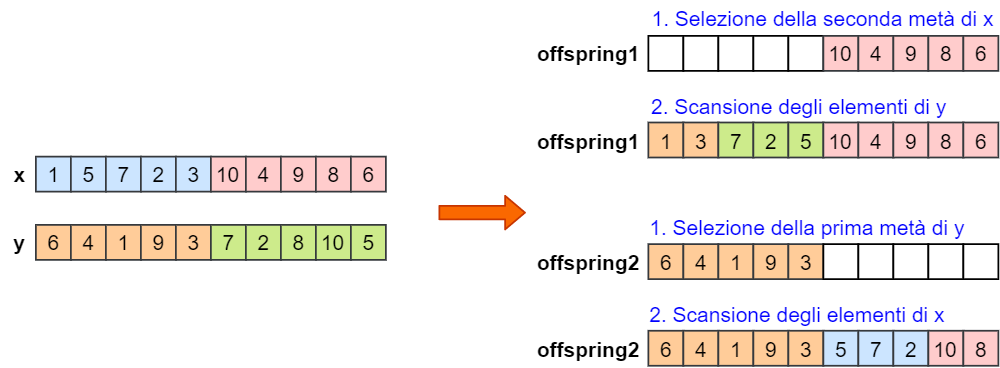
\includegraphics[scale=0.37]{Images/crossover}
  \caption{\footnotesize{Esempio di applicazione del crossover su due istanze x e y.}}
  \label{crossover}
\end{center}
\end{figure}

\begin{algorithm}[h]
\DontPrintSemicolon
\KwIn {$\mathtt{population}$= popolazione di numerosi tour generati mediante un algoritmo di costruzione\newline
$\mathtt{sum\_fitnesses}$= somma delle fitness di tutti gli individui della popolazione\newline
$\mathtt{best\_cost}$= costo della migliore soluzione attuale\newline}
\KwOut {$\mathtt{offspring1, offspring2}$= nuovo individuo generato nella popolazione}
\BlankLine
$\mathtt{n} \gets$ numero di nodi dell'istanza tsp\;
\BlankLine
$\mathtt{x=\{x_1,...,x_n\}\gets} RANDOM(population)$\;
 \BlankLine
 $\mathtt{begin} \gets RANDOM(\{1,...,n/2\})$\;
 $\mathtt{end} \gets RANDOM(\{n/2+1,...,n\})$\;  
 \BlankLine
 \For{$\mathtt{i}\gets begin$ \KwTo $end$}{
	\BlankLine
	$\mathtt{offspring[}i\mathtt{]}\gets x[end - i + begin]$\;
 }  
 
 \If{$cost(offspring) < best\_cost$}{
 	$\mathtt{best\_cost} \gets cost(offspring)$\;
 }
\caption{Mutazione}
\end{algorithm}

\begin{figure}[h]
\begin{center} 
  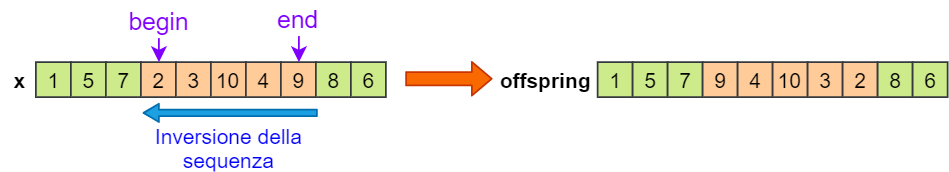
\includegraphics[scale=0.4]{Images/mutation}
  \caption{\footnotesize{Esempio di applicazione della mutazione su un'istanza x.}}
  \label{mutation}
\end{center}
\end{figure}
\chapter{Performance}\label{PERF_PROF}
Le metriche di confronto, utilizzate nell'analisi degli algoritmi, sono il tempo complessivo di creazione e risoluzione del modello ed il costo della soluzione ottenuta. Ciascuna modalità di risoluzione viene applicata a diverse istanze di TSPlib, con un numero differente di nodi.  
\section{Performance variabilty}
Nel corso degli anni '90, gli ingegneri di CPLEX scoprirono che il tempo di risoluzione variasse significativamente in diversi sistemi operativi. Con alcune istanze, le performance migliori si avevano su UNIX mentre con altre su Windows.\\
Il motivo di tale comportamento venne in seguito studiato ed attribuito alla diversa scelta effettuata dai sistemi operativi nel decretare l'ordine delle variabili su cui viene svolto l'albero decisionale.\\
Le scelte svolte inizialmente, nella definizione dei primi nodi dell'albero, si ripercuotono sulla sua successiva evoluzione.\\
Proprio per questo motivo, su alcune istanze, UNIX riusciva a risolvere il problema in tempo minore rispetto a Windows, mentre su altre accadeva l'opposto.\\
Da questi studi, evinse che il Branch and Cut è un sistema caotico e che quindi piccole variazioni delle condizioni iniziali generano grandi differenze nei risultati finali.\\
Per questo motivo, alcuni algoritmi prensentati in questo report, sono stati studiati al variare di alcune condizioni iniziali:
\begin{itemize}
\item{\textbf{Random Seed}\\
definisce il seme da cui CPLEX genera una sequenza di numeri pseudo-casuali (vedi Sezione \ref{param}). Nel momento in cui CPLEX nota che diverse variabili frazionarie hanno lo stesso valore, il risolutore sceglie casualmente su quale di queste applicare il Branch.}
\item{\textbf{Gap}\\
intervallo massimo, tra il valore della migliore funzione obiettivo intera e il valore della funzione di costo del miglior nodo rimanente, che permette di decretare il raggiungimento dell'ottimo secondo CPLEX (vedi Sezione \ref{param}).}
\end{itemize}
La variazione del primo di questi parametri permette di apportare significative modifiche al tempo di risoluzione, non modficando la reale ottimalità della soluzione.\\
La variazione dell'altro parametro permette invece di ottenere una soluzione euristica, ovvero un'approssimazione più lasca di quella ottima.
 
\section{Analisi tabulare}
Un metodo non molto efficiente per lo studio delle performance degli algoritmi, utilizza una struttura tabulare in cui viene inserita una riga per ogni istanza del problema.\\ Inoltre vengono riportati i tempi di esecuzione degli algoritmi su ognuno dei grafi analizzati. Nell'ultima riga per ciascun algoritmo viene riportata la media geometrica dei suoi tempi di esecuzione (vedi esempio in Tabella \ref{result_table}).\\
Solitamente viene impostato un TIME LIMIT uguale per tutti gli algoritmi. Questo rappresenta nella tabella il valore del tempo di esecuzione per un algoritmo che ha impiegato un tempo maggiore o uguale a TIME LIMIT. Spesso viene dato più peso al TIME LIMIT, inserendolo nella tabella con, ad esempio, peso 10 (ovvero TIME LIMIT*10).\\ La debolezza di tale calcolo delle performance risiede nel fatto che non sempre la media descrive  l'efficienza di un soluzione. Infatti non influisce unicamente il tempo di risoluzione del modello ma anche quello necessario alla sua creazione. 

\begin{table}[h]
\centering
\begin{tabular}{|c|c|c|c|}
\multicolumn{1}{c}{\textbf{Istanza}} & \multicolumn{1}{c}{\textbf{Sequential}} & \multicolumn{1}{c}{\textbf{Flow}} &
\multicolumn{1}{c}{\textbf{Loop}}\\
\hline
\textbf{att48} & {212.3} & {12.5} & {4.3}\\
\hline
{\textbf{...}} & {...} & {...} & {...}\\
\hline
\textbf{a280} & {3200} & {2500.8} & {1300.5}\\
\hline
\hline
\multicolumn{1}{c}{} & \multicolumn{1}{c}{2120.3} & \multicolumn{1}{c}{1800.3}& \multicolumn{1}{c}{1000.4}\\
\end{tabular}
\caption{\footnotesize{Tabella di performance con \textbf{TIME LIMIT=3200}.}}\label{result_table}
\end{table}

\section{Performance profiling}
Questo metodo prevede la classificazione dei tempi di esecuzione degli algoritmi in base al numero percentuale di successi, rispetto a un fattore moltiplicativo (ratio) del tempo di esecuzione (vedi Figura \ref{perf_profile}).\\
L'andamento del performance profile di un algoritmo è monotono crescente. Il valore assunto per ogni ratio dagli algoritmi all'interno del grafico è la percentuale del numero di istanze che l'algoritmo risolve con quel fattore rispetto all'ottimo di quel caso.\\
Spesso questi grafici vengono rappresentati in scala logaritmica per notare al meglio le differenze ed avere una migliore raffigurazione.\\
\begin{figure}[h] 
\begin{center} 
  % Requires \usepackage{graphicx} 
  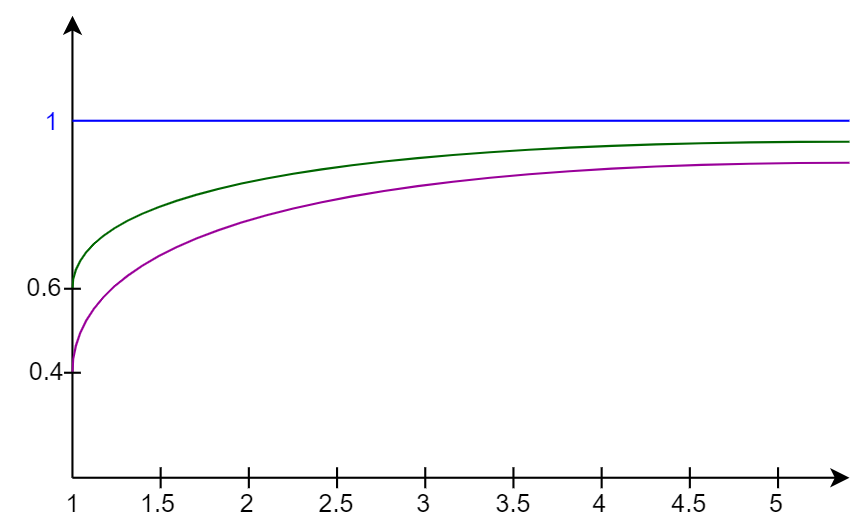
\includegraphics[scale=0.3]{Images/perf_profile} 
  \caption{\footnotesize{Performance profile di due algoritmi.}}
  \label{perf_profile} 
\end{center} 
\end{figure}
Per creare il performance profile degli algoritmi implementati, è stato utilizzato il programma python riportato nella Sezione \ref{perf_profile_py}. 

\section{Analisi degli algoritmi sviluppati}
Nella seguente sezione vengono riportati i grafici relativi ai risultati ottenuti con le implementazioni degli algoritmi descritti nei precedenti capitoli. I valori ottenuti ed utilizzati per realizzare le immagini contenute in questa sezione, sono consultabili nell'Appendice \ref{results}.
\subsection{Algoritmi esatti}
Gli algoritmi basati sul modello compatto, sono stati testati con un time limit di 20 minuti sulle seguenti istanze:
\begin{center}
\begin{multicols}{3}
\begin{itemize}
\item{att48.tsp}
\item{berlin52.tsp}
\item{burma14.tsp}
\item{eil101.tsp}
\item{eil51.tsp}
\item{eil76.tsp}
\item{gr96.tsp}
\item{kroA100.tsp}
\item{kroB100.tsp}
\item{kroB150.tsp}
\item{kroC100.tsp}
\item{kroD100.tsp}
\item{kroE100.tsp}
\item{pr124.tsp}
\item{pr136.tsp}
\item{pr76.tsp}
\item{rat99.tsp}
\item{rd100.tsp}
\item{st70.tsp}
\item{ulysses16.tsp}
\end{itemize}
\end{multicols}
\end{center}
Visionando il performance profile in Figura \ref{pp_compact}, risulta evidente come l'aggiunta dei vincoli come lazy constraint, nel metodo di Miller, Tucker e Zemlin, garantisca un notevole miglioramento delle prestazioni rispetto alla versione originale.\\
\begin{figure}[H] 
\begin{center} 
  % Requires \usepackage{graphicx} 
  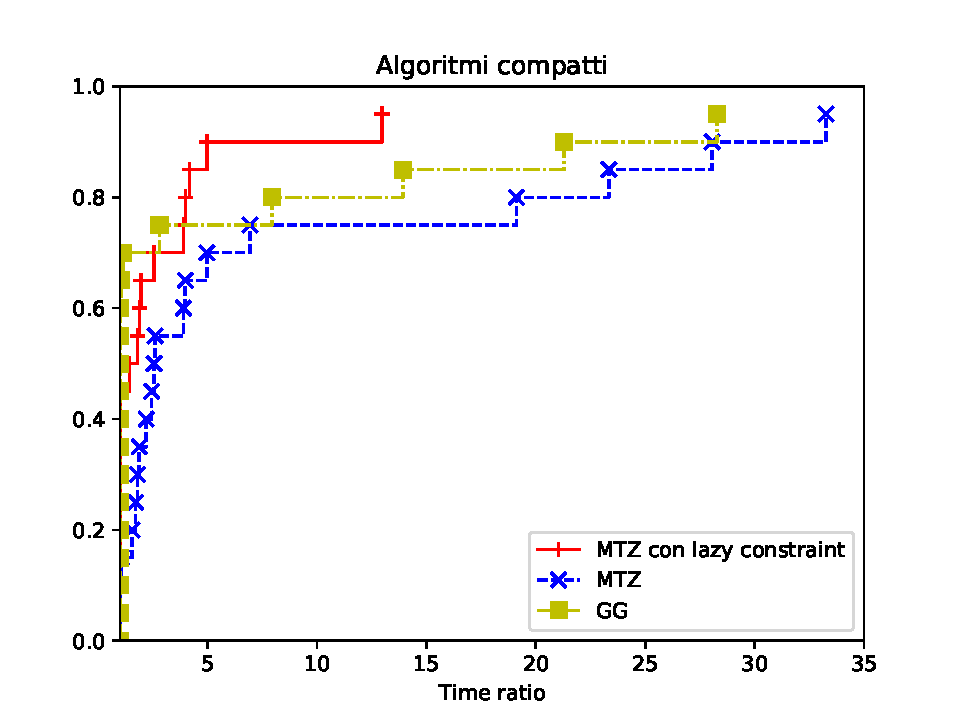
\includegraphics[scale=0.7]{Images/pp_compact}\\ 
  \caption{\footnotesize{Performance profile degli algoritmi compatti.}}
  \label{pp_compact} 
\end{center} 
\end{figure}
Gli algoritmi esatti, che non prevedono l'uso di modelli compatti, sono invece stati testati con un time limit di 10 minuti sul seguente dataset:
\begin{center}
\begin{multicols}{4}
\begin{itemize}
\item{a280.tsp}
\item{ali535.tsp}
\item{att48.tsp}
\item{att532.tsp}
\item{berlin52.tsp}
\item{bier127.tsp}
\item{burma14.tsp}
\item{ch130.tsp}
\item{ch150.tsp}
\item{d198.tsp}
\item{d493.tsp}
\item{d657.tsp}
\item{eil51.tsp}
\item{eil76.tsp}
\item{eil101.tsp}
\item{fl417.tsp}
\item{gil262.tsp}
\item{gr96.tsp}
\item{gr137.tsp}
\item{gr202.tsp}
\item{gr229.tsp}
\item{gr431.tsp}
\item{gr666.tsp}
\item{kroA100.tsp}
\item{kroA150.tsp}
\item{kroA200.tsp}
\item{kroB100.tsp}
\item{kroB150.tsp}
\item{kroB200.tsp}
\item{kroC100.tsp}
\item{kroD100.tsp}
\item{kroE100.tsp}
\item{lin105.tsp}
\item{lin318.tsp}
\item{p654.tsp}
\item{pcb442.tsp}
\item{pr76.tsp}
\item{pr107.tsp}
\item{pr124.tsp}
\item{pr136.tsp}
\item{pr144.tsp}
\item{pr152.tsp}
\item{pr226.tsp}
\item{pr299.tsp}
\item{pr439.tsp}
\item{rat99.tsp}
\item{rat195.tsp}
\item{rat575.tsp}
\item{rat783.tsp}
\item{rd100.tsp}
\item{rd400.tsp}
\item{st70.tsp}
\end{itemize}
\end{multicols}
\end{center}
Dall'analisi dei risultati ottenuti (Figura \ref{pp_exact}), è evidente come l'utilizzo del Branch \& Cut permetta di ottenere prestazioni migliori, ma soprattutto come l'utilizzo delle callback generiche abbia permesso di migliorare notevolmente le prestazioni, rispetto alla versione priva di esse.\\
L'utilizzo del patching ha avuto maggior effetto soprattutto nella prima parte dell'esecuzione del programma, in cui risulta essere molto di aiuto per CPLEX nel raggiungere l'ottimo. Successivamente le soluzioni passate al risolutore MIP, mediante le heuristic callback, vengono scartate da quest'ultimo sempre più spesso.\\
\begin{figure}[H] 
\begin{center} 
  % Requires \usepackage{graphicx} 
  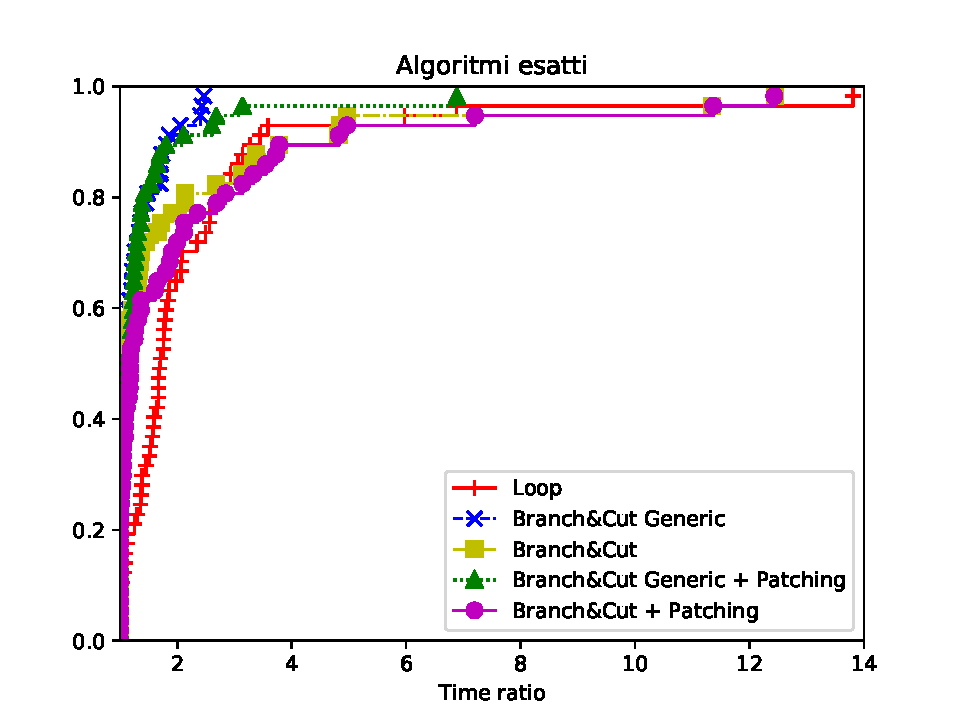
\includegraphics[scale=0.75]{Images/pp_exact}\\ 
  \caption{\footnotesize{Performance profile dei tempi di esecuzione degli algoritmi esatti implementati.}}
  \label{pp_exact} 
\end{center} 
\end{figure}
In Figura \ref{pp_random_seed} viene confrontato invece l'algoritmo loop attraverso l'utilizzo di diversi seed, ponendo l'attenzione su come la performance variability influenzi le prestazioni delle varie soluzioni implementative.
Il performance profile riportato in Figura \ref{pp_gap} confronta i risultati ottenuti mediante l'utilizzo dell'algoritmo loop nella sua versione classica con quelli ottenuti applicando la sua versione euristica. Nel grafico realizzato, le varianti euristiche individuano inizialmente una soluzione utilizzando il gap relativo evidenziato 
nel grafico ed in seguito impostano nuovamente il gap al valore di default ed individuano la soluzione ottima.
\begin{figure}[H] 
\begin{center} 
  % Requires \usepackage{graphicx} 
  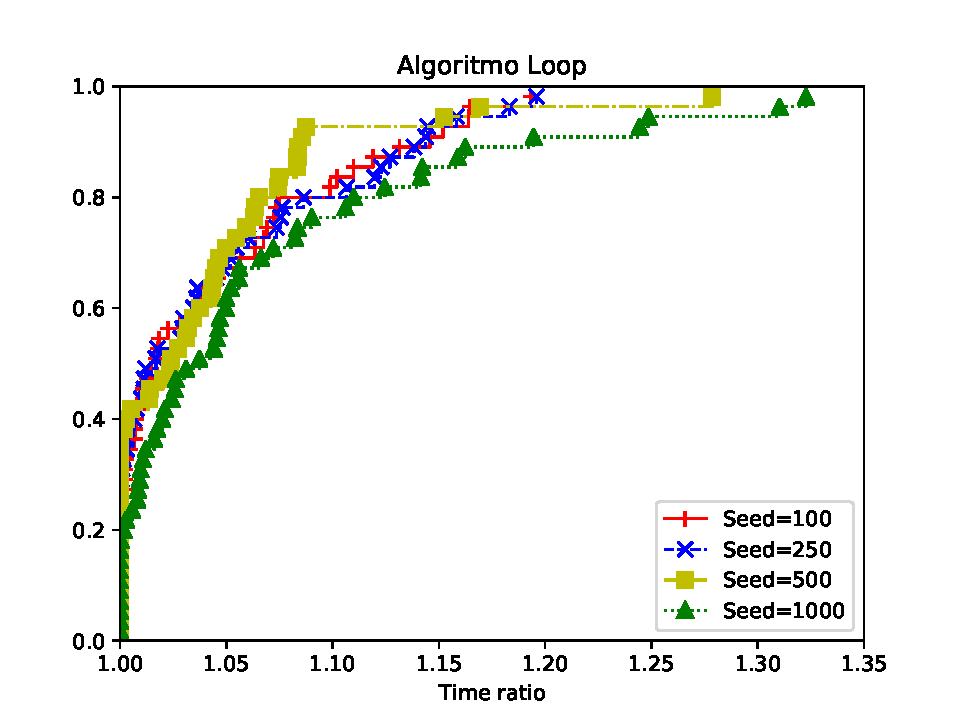
\includegraphics[scale=0.7]{Images/pp_random_seed}\\ 
  \caption{\footnotesize{Performance profile dei tempi di esecuzione dell'algoritmo loop al variare del seed.}}
  \label{pp_random_seed} 
\end{center} 
\end{figure}
\begin{figure}[H] 
\begin{center} 
  % Requires \usepackage{graphicx} 
  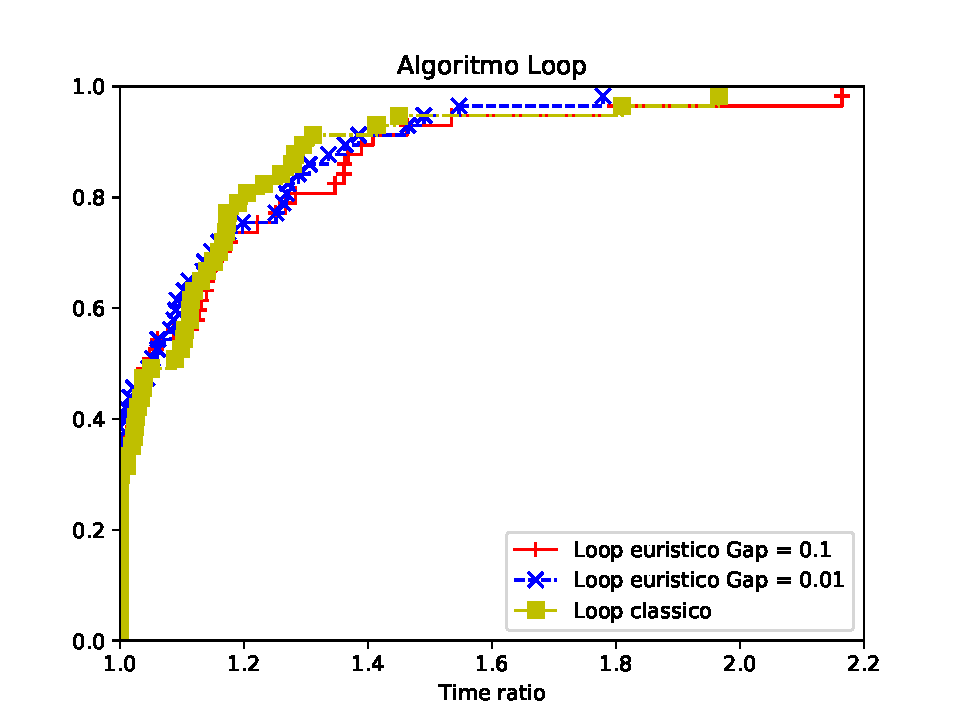
\includegraphics[scale=0.7]{Images/pp_gap}\\ 
  \caption{\footnotesize{Performance profile dei tempi di esecuzione dell'algoritmo loop euristico al variare del gap.}}
  \label{pp_gap} 
\end{center} 
\end{figure}

\vspace{2cm}
\subsection{Algoritmi math-euristici}
Gli algoritmi math-euristici sviluppati sono stati testati sul seguente insieme di istanze, con un time limit 10 minuti:
\begin{center}
\begin{multicols}{3}
\begin{itemize}
\item{a280.tsp}  
\item{att532.tsp} 
\item{bier127.tsp}
\item{d198.tsp}   
\item{d493.tsp}   
\item{eil76.tsp}  
\item{eil101.tsp} 
\item{fl417.tsp}  
\item{gr137.tsp}  
\item{gr202.tsp}  
\item{lin105.tsp} 
\item{lin318.tsp} 
\item{pcb442.tsp} 
\item{pr144.tsp}  
\item{pr264.tsp}  
\item{pr299.tsp}  
\item{pr439.tsp}  
\item{rat575.tsp} 
\item{rd400.tsp}  
\item{u159.tsp}
\end{itemize}
\end{multicols}
\end{center}
Analizzando i risultati ottenuti in Figura \ref{pp_math-heuristic} e \ref{pp_math-heuristic_zoom}) risulta evidente come le prestazioni dell'algoritmo Hard fixing siano migliori, sia nella variante che utilizza le callback generiche che in quella che non ne fa uso, rispetto ad entrambe le soluzioni ottenute dal Soft fixing.
\begin{figure}[h] 
\begin{center} 
  % Requires \usepackage{graphicx} 
  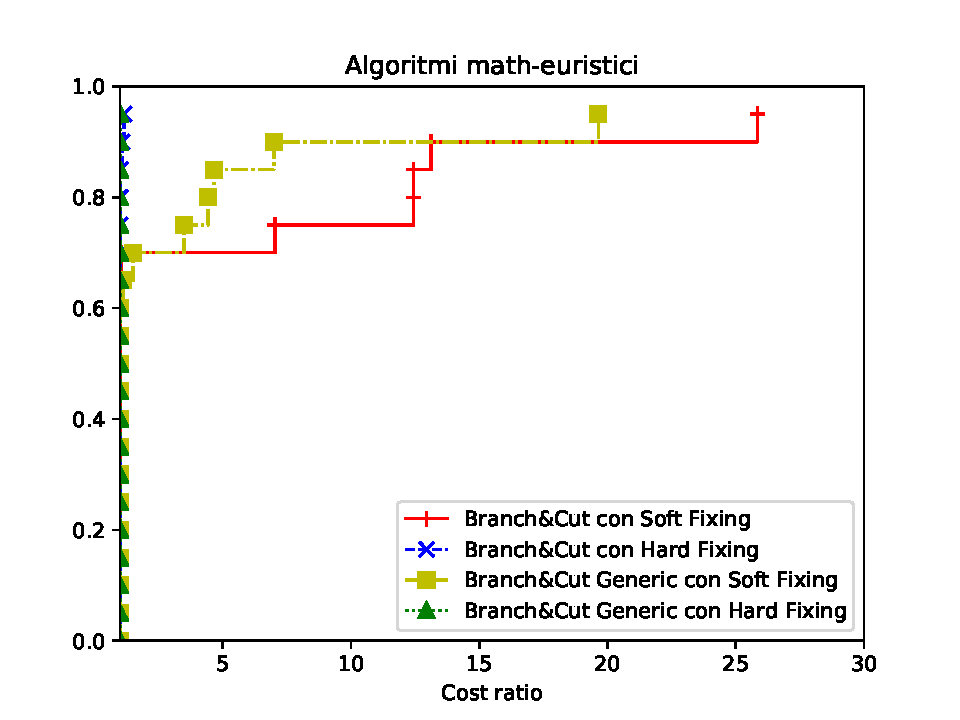
\includegraphics[scale=0.8]{Images/pp_math-heuristic}\\ 
  \caption{\footnotesize{Confronto degli algoritmi math-euristici in base al costo della soluzione ottenuta.}}
  \label{pp_math-heuristic} 
\end{center} 
\end{figure}

\begin{figure}[h] 
\begin{center} 
  % Requires \usepackage{graphicx} 
  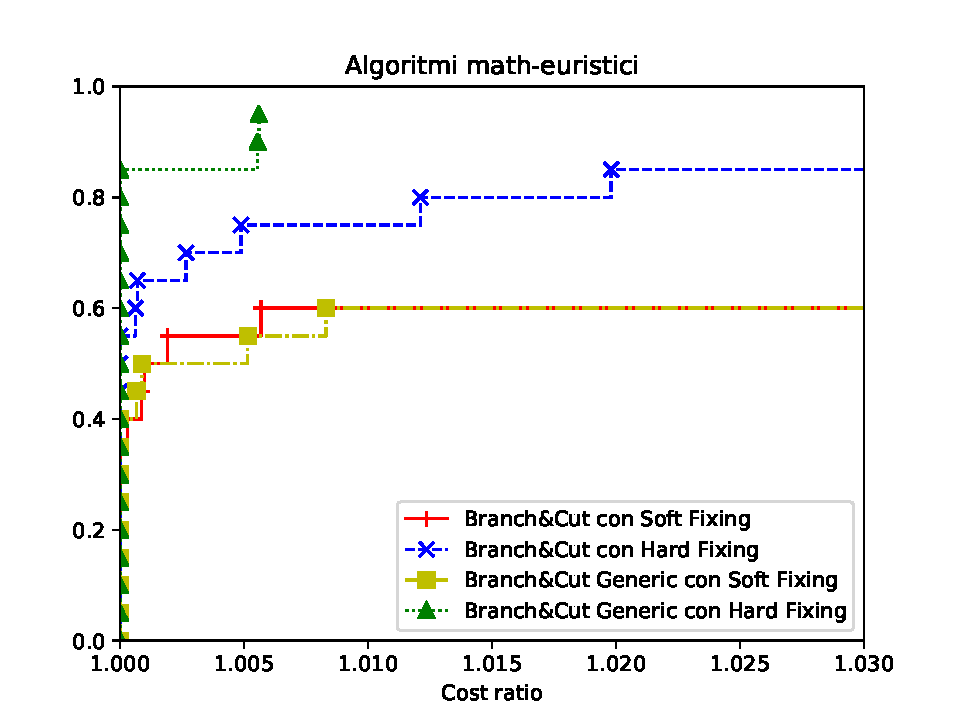
\includegraphics[scale=0.8]{Images/pp_math-heuristic_zoom}\\ 
  \caption{\footnotesize{Dettaglio del confronto degli algoritmi math-euristici in base al costo della soluzione ottenuta.}}
  \label{pp_math-heuristic_zoom} 
\end{center} 
\end{figure}
\vspace{10cm}
\subsection{Algoritmi euristici}
\subsubsection{Multi-start}\label{construction_perf}
In questa prima sezione, vengono analizzati i diversi algoritmi di costruzione implementati, applicando l'algoritmo multistart sulle seguenti istanze:
\begin{center}
\begin{multicols}{4}
\begin{itemize}
\item{a280.tsp}
\item{ali535.tsp}
\item{att532.tsp}
\item{d1291.tsp}
\item{d1665.tsp}
\item{d2103.tsp}
\item{d493.tsp}
\item{d657.tsp}
\item{dsj1000.tsp}
\item{fl1400.tsp}
\item{fl1577.tsp}
\item{fl417.tsp}
\item{gil262.tsp}
\item{gr431.tsp}
\item{gr666.tsp}
\item{lin318.tsp}
\item{nrw1379.tsp}
\item{p654.tsp}
\item{pcb1173.tsp}
\item{pcb442.tsp}
\item{pr1002.tsp}
\item{pr299.tsp}
\item{pr439.tsp}
\item{rat575.tsp}
\item{rat783.tsp}
\item{rd400.tsp}
\item{rl1304.tsp}
\item{rl1323.tsp}
\item{rl1889.tsp}
\item{u1060.tsp}
\item{u1432.tsp}
\item{u1817.tsp}
\item{u574.tsp}
\item{u724.tsp}
\item{vm1084.tsp}
\item{vm1748.tsp}
\end{itemize}
\end{multicols}
\end{center}

In Figura \ref{pp_construction}, viene riportato il performance profile ottenuto dall'esecuzione dell'algoritmo multistart, generando 40 differenti soluzioni per ciascuna istanza del problema e restituendo solo il costo della migliore tra queste.\\
Le soluzioni di costo minore sono quelle restituite dall'algoritmo Nearest Neighborhood, in particolare con l'aggiunta del metodo GRASP. 
Inoltre si è notato come il tempo necessario alla definizione di una soluzione mediante il metodo insertion sia molto elevato. 
\begin{figure}[h] 
\begin{center} 
  % Requires \usepackage{graphicx} 
  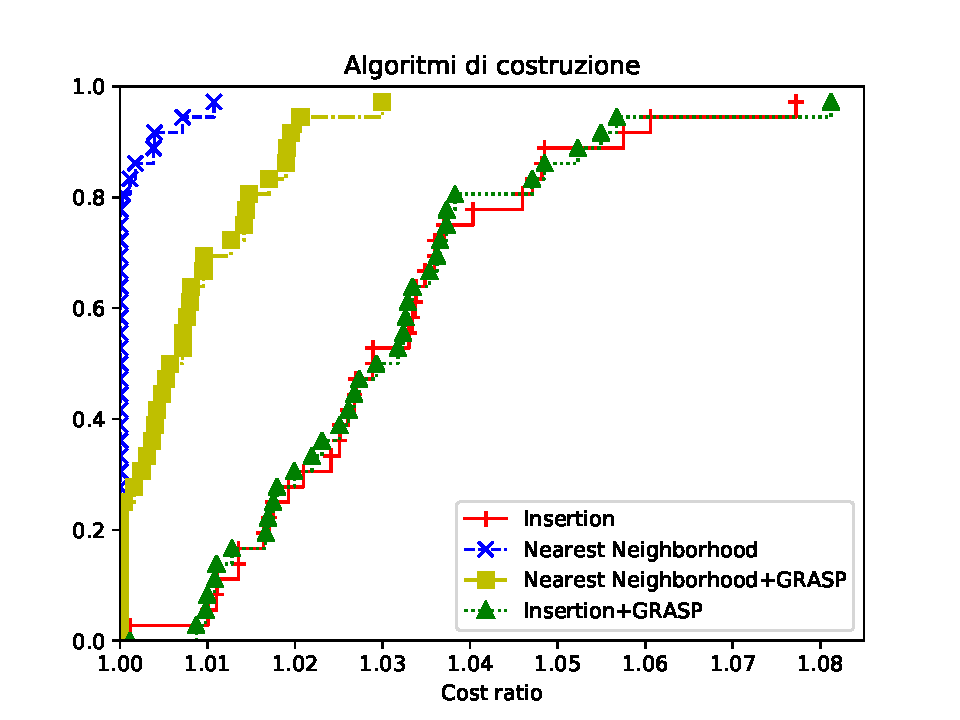
\includegraphics[scale=0.8]{Images/pp_construction}\\ 
  \caption{\footnotesize{Confronto dei vari multistart in base all'algoritmo di costruzione utilizzato.}}
  \label{pp_construction} 
\end{center} 
\end{figure}
\subsubsection{Algoritmi meta-euristici}
Tutti gli algoritmi meta-euristici sviluppati, escluso il genetico, prevedono la possibilità di utilizzare uno qualsiasi tra gli algoritmi di costruzione definiti, semplicemente associando specifici valori a delle macro.\\
Per i motivi descritti nella sezione precedente, gli algoritmi sono stati testati però utilizzando il metodo di costruzione Nearest Neighborhood e con un time limit di 10 minuti. In questi test, è stata impostata una macro che permette al multistart di essere eseguito in multithreading in questo intervallo di tempo, generando iterativamente 8 soluzioni alla volta. Il primo dataset su cui sono stati svolti i test è il seguente:
\begin{center}
\begin{multicols}{3}
\begin{itemize}
\item{d1291.tsp}
\item{d1655.tsp} 
\item{d2103.tsp} 
\item{dsj1000.tsp}
\item{fl1400.tsp} 
\item{fl1577.tsp} 
\item{nrw1379.tsp} 
\item{pcb1173.tsp} 
\item{pr1002.tsp}
\item{pr2392.tsp}
\item{rl1304.tsp}
\item{rl1323.tsp}
\item{rl1889.tsp}
\item{u1060.tsp} 
\item{u1432.tsp}
\item{u1817.tsp}
\item{u2152.tsp}
\item{u2319.tsp}
\item{vm1084.tsp}
\item{vm1748.tsp}
\end{itemize}
\end{multicols}
\end{center}
L'algoritmo genetico non è stato applicato a questo primo dataset. Il motivo di tale scelta, riguarda il tempo di calcolo troppo elevato per la generazione della popolazione.\\
Per tale motivo tutti gli algoritmi meta-euristici sono stati testati nuovamente sulle seguenti istanze di dimensione minore, per ottenere un confronto più equo della soluzione del genetico con le altre:
\begin{center}
\begin{multicols}{3}
\begin{itemize}
\item{a280.tsp}
\item{bier127.tsp}
\item{ch130.tsp}
\item{ch150.tsp}
\item{d198.tsp}
\item{gil262.tsp}
\item{gr137.tsp}
\item{kroA150.tsp}
\item{kroA200.tsp}
\item{kroB150.tsp}
\item{kroB200.tsp}
\item{pr124.tsp}
\item{pr136.tsp}
\item{pr144.tsp}
\item{pr152.tsp}
\item{pr226.tsp}
\item{pr264.tsp}
\item{pr299.tsp}
\item{rd400.tsp}
\item{u159.tsp}
\end{itemize}
\end{multicols}
\end{center}
Analizzando i risultati ottenuti in entrambi i test (Figura \ref{pp_heuristic} e \ref{pp_genetic}), le soluzioni con costo minore sono quelle ottenute mediante il Simulated Annealing e il VNS ibribo. Nel primo caso, con istanze di grandezza maggiore, la seconda implementazione del VNS genera soluzioni di costo minore mentre nel confronto con l'algoritmo genetico, la prima implementazione del VNS risulta migliore.\\
I grafici in Figura \ref{cost_vns}, \ref{cost_tabu}, \ref{cost_sa} e \ref{cost_genetic} rappresentano invece l'andamento del costo applicando rispettivamente il VNS ibrido, il Tabu Search, il Simulated Annealing e l'algoritmo genetico all'istanza \textit{bier127.tsp}.
\begin{figure}[h] 
\begin{center} 
  % Requires \usepackage{graphicx} 
  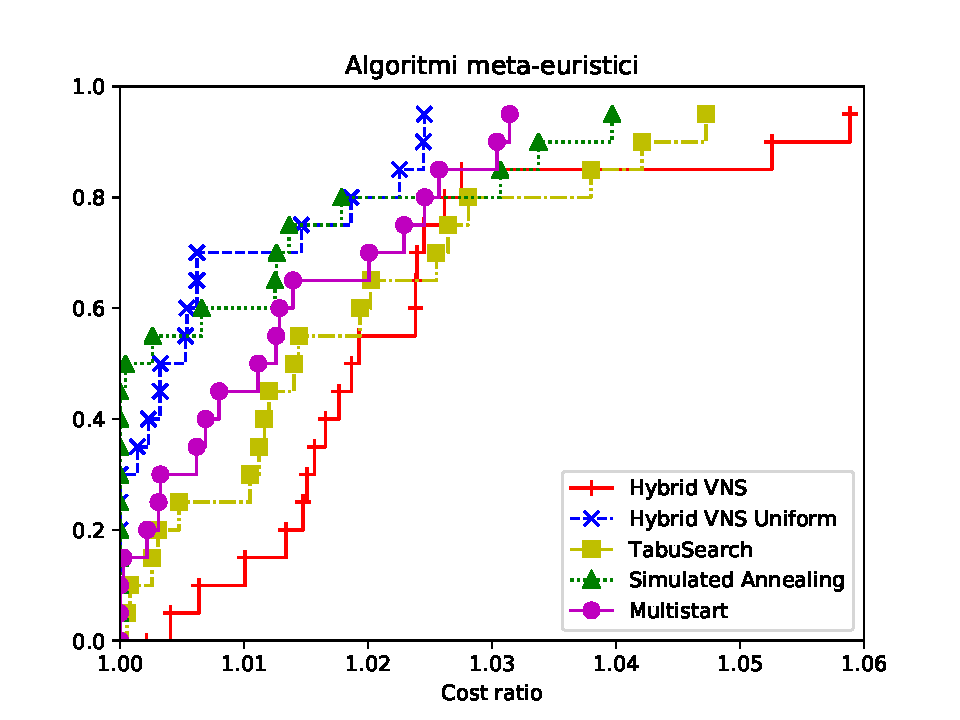
\includegraphics[scale=0.8]{Images/pp_heuristic}\\ 
  \caption{\footnotesize{Confronto dei costi delle soluzioni ottenute mediante gli algoritmi meta-euristici, escluso il genetico.}}
  \label{pp_heuristic} 
\end{center}
\end{figure}
\begin{figure}[h] 
\begin{center} 
  % Requires \usepackage{graphicx} 
  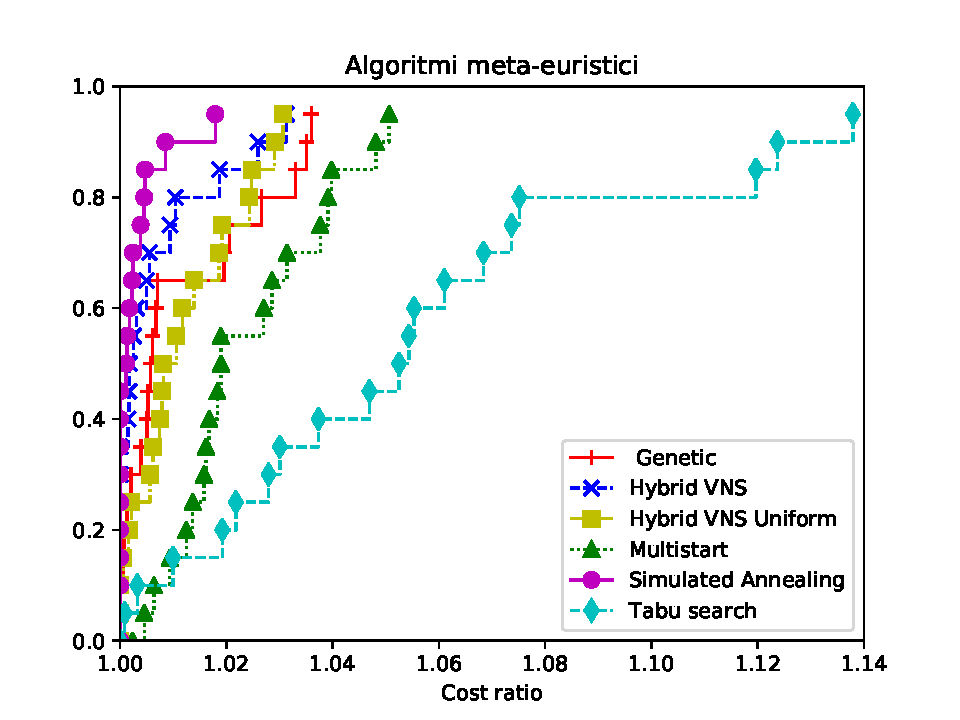
\includegraphics[scale=0.8]{Images/pp_genetic}\\ 
  \caption{\footnotesize{Confronto dei costi delle soluzioni ottenute mediante tutti gli algoritmi meta-euristici.}}
  \label{pp_genetic} 
\end{center} 
\end{figure}
\begin{figure}[h]
\begin{center} 
  % Requires \usepackage{graphicx} 
  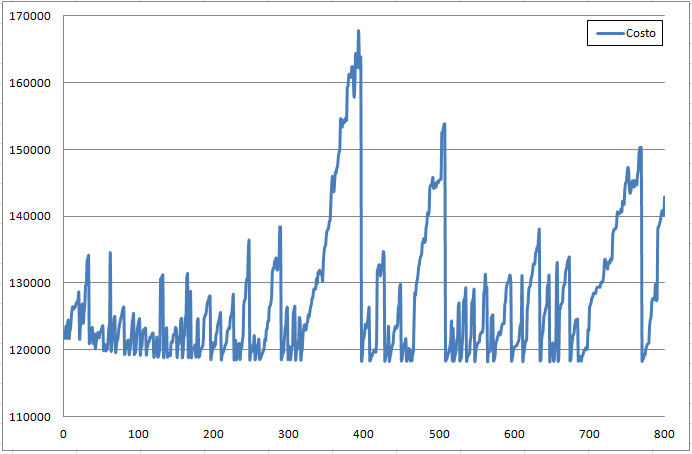
\includegraphics[scale=0.7]{Images/cost_vns}\\ 
  \caption{\footnotesize{Evoluzione del costo della soluzione attuale nell'algoritmo VNS.}}
  \label{cost_vns} 
\end{center} 
\end{figure}
\begin{figure}[h] 
\begin{center} 
  % Requires \usepackage{graphicx} 
  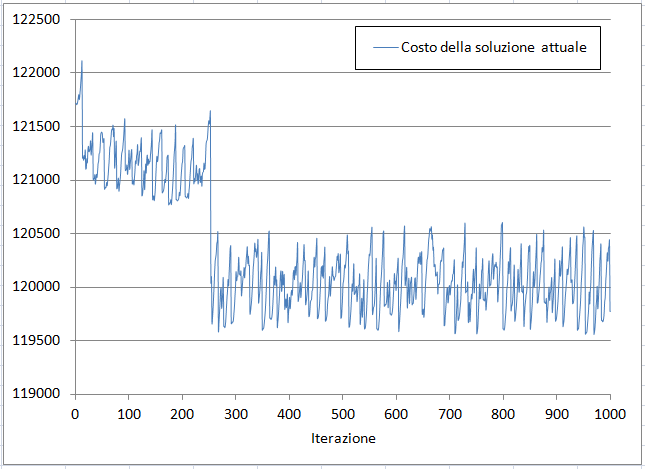
\includegraphics[scale=0.7]{Images/cost_tabu}\\ 
  \caption{\footnotesize{Evoluzione del costo della soluzione attuale nell'algoritmo Tabu search.}}
  \label{cost_tabu} 
\end{center} 
\end{figure}
\begin{figure}[h] 
\begin{center} 
  % Requires \usepackage{graphicx} 
  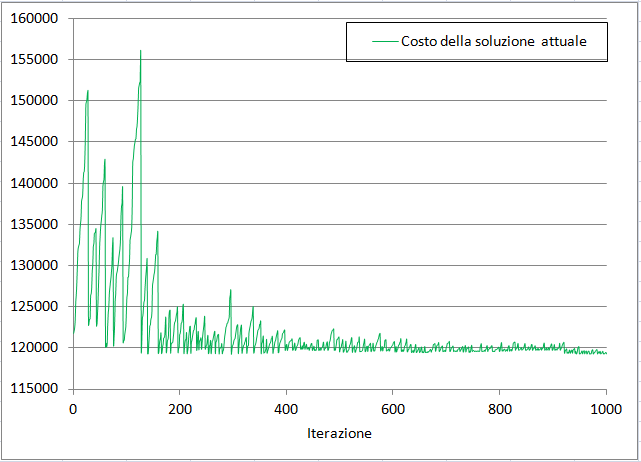
\includegraphics[scale=0.7]{Images/cost_sa}\\ 
  \caption{\footnotesize{Evoluzione del costo della soluzione attuale nell'algoritmo Simulated Annealing.}}
  \label{cost_sa} 
\end{center} 
\end{figure}
\begin{figure}[h]
\begin{center} 
  % Requires \usepackage{graphicx} 
  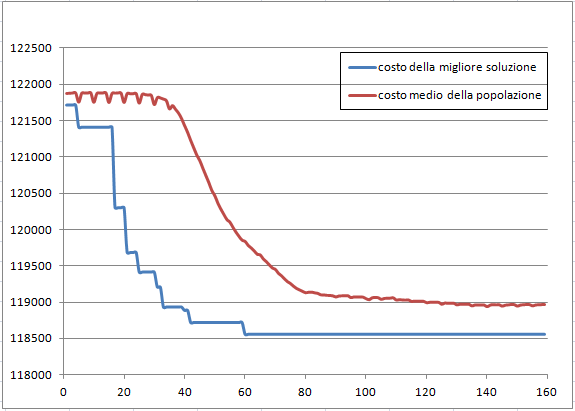
\includegraphics[scale=0.7]{Images/cost_genetic}\\ 
  \caption{\footnotesize{Evoluzione del costo medio della popolazione e del costo della soluzione migliore nell'algoritmo genetico.}}
  \label{cost_genetic} 
\end{center} 
\end{figure}
\appendix
\input{Chapters/TSPLIB.tex}
\chapter{ILOG CPLEX}
In questa sezione verranno approfondite alcune funzioni di CPLEX necessarie ad implementare gli algoritmi descritti nei capitoli precedenti.

\section{Funzionamento}
Per poter utilizzare gli algoritmi di risoluzione forniti da CPLEX è necessario costruire il modello matematico del problema, legato all'istanza precedentemente descritta.\\
CPLEX ha due meccanismi di acquisizione dell'istanza:
\begin{enumerate}
\item{\textbf{modalità interattiva:}\\
in cui il modello viene letto da un file precedentemente generato (\textit{model.lp})}
\item{\textbf{creazione nel programma:}\\
il modello viene creato attraverso le API del linguaggio usato per la scrittura del programma}
\end{enumerate}

Le strutture utilizzate da CPLEX sono due (vedi Figura \ref{strutture_cplex}):
\begin{itemize}
\item{\textbf{ENV:} contiene i parametri necessari all'esecuzione e al salvataggio dei risultati}
\item{\textbf{LP:} contiene il modello che viene analizzato da CPLEX durante la computazione del problema di ottimizzazione}
\end{itemize}

\begin{figure}[h] 
\begin{center} 
  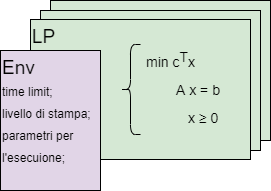
\includegraphics[scale=0.7]{Images/cplex_structs}\\ 
  \caption{\footnotesize{Strutture CPLEX}}
  \label{strutture_cplex} 
\end{center} 
\end{figure}

Ad ogni ENV è possibile associare più LP, in modo da poter risolvere in parallelo più problemi di ottimizzazione, ma nel nostro caso ne sarà sufficiente solo uno.\\
Per convenzione è stato deciso di etichettare i rami $(i,j)$ dell'istanza rispettando la proprietà $i<j$. In Figura \ref{Indici_matrice} è riportato lo schema degli indici che vengono utilizzati per etichettare le variabili.\\
In questa figura le celle $(i,j)$ bianche, sono quelle effettivamente utilizzate per indicare un arco secondo la convenzione. Il numero all'interno di queste caselle rappresenta invece l'ordine in cui queste variabili vengono inserite nel modello e quindi gli indici associati da CPLEX per accedere alla soluzione.\\
\begin{figure}[h] 
\begin{center} 
  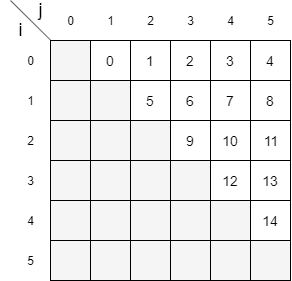
\includegraphics[scale=0.6]{Images/indices_matrix}\\ 
  \caption{\footnotesize{Indici della matrice}}
  \label{Indici_matrice} 
\end{center} 
\end{figure}

\section{Funzioni}
\subsection{Costruzione e modifica del modello}
Per poter costruire il modello da analizzare, come prima cosa, è necessario creare un puntatore alle due strutture dati utilizzate da CPLEX.
\lstinputlisting[caption={\footnotesize{modelTSP.txt}}, style=code, firstnumber=1, firstline=27, lastline=29, label=tsp_model, language=c]{Source/modelTSP.txt}
La funzione alla riga 2 alloca la memoria necessaria e riempie la struttura con valori di default. Nel caso in cui non termini con successo memorizza un codice d'errore in \textit{error}.\\
La funziona invocata nella riga successiva, invece, associa la struttura LP all'ENV che gli viene fornito. Il terzo parametro passato, nell'esempio "TSP", sarà il nome del modello. Al termine di queste operazioni verrà quindi creato un modello vuoto. All'interno del nostro programma per inizializzarlo è stata costruita la seguente funzione:
\begin{center}
\begin{tabular}{c}
\begin{lstlisting}[linewidth=370pt, basicstyle=\footnotesize\sffamily,] 
void cplex_build_model(tsp_instance* tsp_in, CPXENVptr env, CPXLPptr lp);
\end{lstlisting}
\end{tabular}
\end{center}
\begin{table}[h]
\centering
\begin{tabular}{rl}
\textbf{tsp\_in: } & {puntatore alla struttura che contiene l'istanza del problema (letta dal file TSPlib)} \\
\textbf{env: } & {puntatore alla struttura ENV precedentemente creata}\\
\textbf{lp: } & {puntatore alla struttura LP  precedentemente creata}\\
\end{tabular}
\end{table}
All'interno di \textbf{cplex\_build\_model()} viene aggiunta una colonna alla volta al modello, definendo quindi anche la funzione obiettivo. Le variabili aggiunte corrispondono agli archi del grafo e per ciascuno di questi viene calcolato il costo come distanza euclidea. La funzione necessaria ad inserire colonne e definire la funzione di costo è la seguente:
\begin{center}
\begin{tabular}{c}
\begin{lstlisting}[linewidth=400pt, basicstyle=\footnotesize\sffamily,] 
int CPXnewcols( CPXCENVptr env, CPXLPptr lp, int ccnt, double const * obj, 
		double const * lb, double const * ub, char const * xctype, char ** colname);    
\end{lstlisting}
\end{tabular}
\end{center}
\begin{table}[h]
\begin{tabular}{rl}
\textbf{env:} & {puntatore alla struttura ENV precedentemente creata}\\
\textbf{lp:} & {puntatore alla struttura LP precedentemente creata}\\
\textbf{ccnt:} & {numero di colonne da inserire} \\    
\textbf{obj:} & {vettore dei costi relativi agli archi da inserire} \\
\textbf{lb:} & {vettore contenente i lower bound dei valori assumibili dalle variabili da}\\
&{inserire}\\            
\textbf{ub:} & {vettore contenente gli upper bound dei valori assumibili dalle variabili da}\\
&{inserire}\\
\textbf{xctype:} & {vettore contenente la tipologia delle variabili da inserire}\\
\textbf{colname:} & {vettore di stringhe contenenti i nomi delle variabili da inserire}\\
\textbf{Return Value:} & {0 in caso di successo, un valore diverso da 0 se si verifica un errore}\\
\end{tabular}
\end{table}
La generica colonna \textbf{i}, aggiunta dalla funzione, sarà definita dalle informazioni contenute all'interno della posizione \textbf{i} degli array, ricevuti come parametri. Nel programma elaborato durante il corso, viene aggiunta una colonna alla volta all'interno del modello. Per far ciò, è necessario comunque utilizzare riferimenti alle informazioni da inserire, in modo da ovviare il problema riguardante la tipologia di argomenti richiesti, che sono array. Ad esempio, nel nostro caso, la tipologia di una nuova variabile inserita sarà un riferimento al carattere \textbf{'B'}, che la identifica come binaria.\\
Per poter inserire il primo insieme di vincoli del problema\\
$$
\underset{e\in \delta(v)}\sum{\;x_e} = 2\;\;\;\;\;\;\;\;\;\;\;\;\;\;\;\;\;\;\forall\;v\in V \\\\
$$
\\
viene invece sfruttata la seguente funzione:
\begin{center}
\begin{tabular}{c}
\begin{lstlisting}[linewidth=380pt, basicstyle=\footnotesize\sffamily,]  
int CPXnewrows( CPXCENVptr env, CPXLPptr lp, int rcnt, double const * rhs,
		char const * sense, double const * rngval, char ** rowname);   
\end{lstlisting}
\end{tabular}
\end{center}
\begin{table}[h]
\centering
\begin{tabular}{rl}
\textbf{env:} & {puntatore alla struttura ENV precedentemente creata}\\
\textbf{lp:} & {puntatore alla struttura LP precedentemente creata}\\
\textbf{rcnt:} & {numero di righe (vincoli) da inserire}\\
\textbf{rhs:} & {vettore dei termini noti dei vincoli}\\
\textbf{sense:} & {vettore di caratteri che specifica il tipo di vincoli da inserire.}\\
&{Ogni carattere può assumere:}\\
&{\textit{'L'} per vincolo $\leq$}\\
&{\textit{'E'} per vincolo $=$}\\
&{\textit{'G'} per vincolo $\geq$}\\
&{\textit{'R'} per vincolo definito in un intervallo}\\
\textbf{rngval:} & {vettore di range per i valori di ogni vincolo (nel nostro caso è NULL)}\\
\textbf{rowname} & {vettore di stringhe contenenti i nomi delle variabili da inserire}\\
\textbf{Return Value:} & {0 in caso di successo, un valore diverso da 0 se si verifica un errore}\\
\end{tabular}
\end{table}
In modo analogo all'inserimento delle colonne, nel nostro programma viene aggiunta una riga alla volta nel modello. L'\textbf{i}-esima riga aggiunta corrisponderà al vincolo imposto sul nodo \textbf{i}-esimo, imponendo a 1 il coefficiente della variabile $x_{k,j}$ se $k=i \;\wedge j=i$ per ogni variabile del modello. In questo modo però viene aggiunto un vincolo in cui è necessario cambiare i coefficienti delle variabili che ne prendono parte. Per fare ciò è necessaria la funzione:
\begin{center}
\begin{tabular}{c}
\begin{lstlisting}[linewidth=380pt, basicstyle=\footnotesize\sffamily,]   
int CPXchgcoef(CPXCENVptr env, CPXLPptr lp, int i, int j, double newvalue);
\end{lstlisting}
\end{tabular}
\end{center}
\begin{table}[h]
\centering
\begin{tabular}{rl}
\textbf{env:} & {puntatore alla struttura ENV precedentemente creata}\\
\textbf{lp:} & {puntatore alla struttura LP precedentemente creata}\\
\textbf{i:} & {intero che specifica l'indice della riga in cui modificare il coefficiente}\\
\textbf{j:} & {intero che specifica la colonna in cui si trova la variabile di cui modificare}\\
&{il coefficiente}\\
\textbf{newvalue:} & {nuovo valore del coefficiente}\\
\textbf{Return Value:} & {0 in caso di successo, un valore diverso da 0 se si verifica un errore}\\
\end{tabular}
\end{table}
L'utilizzo di questa metodo per inserire nuovi vincoli è però considerato inefficiente. Al suo posto è consigliato l'utilizzo di una funzione che inserisca il vincolo con già i coefficienti delle variabili impostati al valore corretto:
\begin{center}
\begin{tabular}{c}
\begin{lstlisting}[linewidth=400pt, basicstyle=\footnotesize\sffamily,]  
int CPXaddrows( CPXCENVptr env, CPXLPptr lp, int ccnt, int rcnt, int nzcnt,
		double const * rhs, char const * sense, int const * rmatbeg, 
		int const * rmatind, double const * rmatval, char ** colname, 
		char ** rowname );   
\end{lstlisting}
\end{tabular}
\end{center}
\begin{table}[h]
\centering
\begin{tabular}{rl}
\textbf{env:} & {puntatore alla struttura ENV precedentemente creata}\\
\textbf{lp:} & {puntatore alla struttura LP precedentemente creata}\\
\textbf{ccnt:} & {numero di nuove colonne che devono essere aggiunte}\\
\textbf{rcnt:} & {numero di nuove righe che devono essere aggiunte}\\
\textbf{nzcnt:} & {numero di coefficienti non nulli nel vincolo aggiunto}\\
\textbf{rhs:} & {vettore con i termini noti per ogni vincolo da aggiungere}\\
\textbf{sense:} & {vettore con il tipo di vincoli da aggiungere, scelto tra:}\\
&{\textit{'L'} per vincolo $\leq$}\\
&{\textit{'E'} per vincolo $=$}\\
&{\textit{'G'} per vincolo $\geq$}\\
&{\textit{'R'} per vincolo definito in un intervallo}\\
\textbf{rmatbeg:} & {vettore per definire le righe da aggiungere}\\
\textbf{rmatind:} & {vettore per definire le righe da aggiungere}\\
\textbf{rmatval:} & {vettore per definire le righe da aggiungere}\\
\textbf{colname:} & {vettore contenente i nomi delle nuove colonne}\\
\textbf{rowname:} & {vettore contenente i nomi dei nuovi vincoli}\\
\textbf{Return Value:} & {0 in caso di successo, un valore diverso da 0 se si verifica un errore}\\
\end{tabular}
\end{table}
Per rimuovere invece delle righe, viene utilizzata la seguente funzione:
\begin{center}
\begin{tabular}{c}
\begin{lstlisting}[linewidth=330pt, basicstyle=\footnotesize\sffamily,]     
int CPXdelrows( CPXCENVptr env, CPXLPptr lp, int begin, int end );
\end{lstlisting}
\end{tabular}
\end{center}
\begin{table}[h]
\centering
\begin{tabular}{rl}
\textbf{env:} & {puntatore alla struttura ENV precedentemente creata}\\
\textbf{lp:} & {puntatore alla struttura LP precedentemente creata}\\
\textbf{begin:} & {indice numerico della prima riga da cancellare}\\
\textbf{end:} & {indice numerico dell'ultima riga da cancellare}\\
\textbf{Return Value:} & {0 in caso di successo, un valore diverso da 0 se si verifica un errore}\\
\end{tabular}
\end{table} 
\vspace{2 cm}
Per poter impostare una variabile $x_{i,j}$ ad una valore fissato è necessario rendere i suoi lower e upper bound alla quantità voluta. Per cambiare questi parametri viene utilizzata la seguente funzione: 
\begin{center}
\begin{tabular}{c}
\begin{lstlisting}[linewidth=375pt, basicstyle=\footnotesize\sffamily,]   
int CPXchgbds(CPXCENVptr env, CPXLPptr lp, int cnt, const int * indices, 
		const char * lu, const double * bd); 
\end{lstlisting}
\end{tabular}
\end{center}
\begin{table}[h]
\centering
\begin{tabular}{rl}
\textbf{env:} & {puntatore alla struttura ENV}\\
\textbf{lp:} & {puntatore alla struttura LP}\\
\textbf{cnt:} & {numero totale di bound da cambiare}\\
\textbf{indices:} & {vettore con gli indice delle colonne corrispondenti alle variabili}\\
&{di cui cambiare il bound}\\
\textbf{lu:} & {array di caratteri che specificano il bound da modificare,}\\
&{a scelta tra:}\\
&{\textit{'U'} per upper bound}\\
&{\textit{'L'} per lower bound}\\
&{\textit{'B'} per entrambi}\\
\textbf{bd:} & {vettore con i nuovi valori}\\
\textbf{Return Value:} & {0 in caso di successo, un valore diverso da 0 se si verifica un errore}\\
\end{tabular}
\end{table}
\subsection{Calcolo della soluzione}
Per ottenere la soluzione ottima del problema di ottimizzazione correlato al modello definito in CPLEX, vengono utilizzate due fasi:
\begin{itemize}
\item{\textbf{Risoluzione del problema di ottimizzazione}\\\\
\begin{tabular}{c}
\begin{lstlisting}[linewidth=220pt, basicstyle=\footnotesize\sffamily,]
int CPXmipopt(CPXCENVptr env, CPXLPptr lp);
\end{lstlisting}
\end{tabular}
\begin{table}[h]
\centering
\begin{tabular}{rl}
\textbf{env:} & {puntatore alla struttura ENV precedentemente creata}\\
\textbf{lp:} & {puntatore alla struttura LP precedentemente creata}\\
\textbf{Return Value:} & {0 in caso di successo, un valore diverso da 0 se si verifica un errore}\\
\end{tabular}
\end{table}
}
\item{\textbf{Ottenimento della soluzione}\\\\
\begin{tabular}{c}
\begin{lstlisting}[linewidth=380pt, basicstyle=\footnotesize\sffamily,]
int CPXgetmipx (CPXENVptr env, CPXLPptr lp, double *x, int begin, int end);
\end{lstlisting}
\end{tabular}
\vspace{2 cm}
\begin{table}[h]
\centering
\begin{tabular}{rl}
\textbf{env:} & {puntatore alla struttura ENV precedentemente creata}\\
\textbf{lp:} & {puntatore alla struttura LP precedentemente creata}\\
\textbf{x:} & {puntatore a un vettore di double in cui verranno salvati i valori}\\
& {delle variabili ottenuti dalla soluzione ottima}\\
\textbf{begin:} & {primo indice della variabile di cui si vuole memorizzare ed analizzare}\\
&{ il valore}\\
\textbf{end:} & {indice dell'ultima variabile di cui si vuole memorizzare ed analizzare}\\
&{il valore}\\
\textbf{Return Value:} & {0 in caso di successo, un valore diverso da 0 se si verifica un errore}\\
\end{tabular}
\end{table}
\\Questa funzione salva in $x$ tutte le variabili che hanno indice $i\in [begin, end]$ e quindi $x$ deve essere un vettore di almeno $end-begin+1$ valori. Nel nostro programma, vengono analizzati i valori di tutte le variabili definite.\\
Per questo motivo \textbf{begin = 0} e 
\textbf{end = num\_colonne - 1}\footnote{numero di variabili=CPXgetnumcols(env,lp);}\footnote{numero di vincoli=CPXgetnumrows(env,lp);}.\\
In seguito il nostro programma analizza la correttezza della soluzione svolgendo la verifica su:
\begin{itemize}
\item{\textit{valori assunti dalle variabili}\\
ciascun $x_{i,j}$ assume valore $0$ o $1$ con una tolleranza di $\epsilon=10^{-5}$}
\item{\textit{grado di ciascun nodo}\\
il tour è composto al massimo da due archi che tocchino lo stesso nodo}
\end{itemize}
}
\item{\textbf{Gap relativo}\\
La seguente funzione permette di ottenere il gap relativo della funzione obiettivo per un'ottimizzazione MIP.\\
\begin{center}
\begin{tabular}{c}
\begin{lstlisting}[linewidth=350pt, basicstyle=\footnotesize\sffamily,]
int CPXgetmiprelgap( CPXCENVptr env, CPXCLPptr lp, double * gap_p );
\end{lstlisting}
\end{tabular}
\end{center}
\begin{table}[h]
\centering
\begin{tabular}{rl}
\textbf{env:} & {puntatore alla struttura ENV precedentemente creata}\\
\textbf{lp:} & {puntatore alla struttura LP precedentemente creata}\\
\textbf{gap\_p:} & {puntatore in cui verrà salvato il gap}\\
\textbf{Return Value:} & {0 in caso di successo, un valore diverso da 0 se si verifica un errore}\\
\end{tabular}
\end{table}
Per un problema di minimizzazione il gap relativo viene calcolato come:
$$\frac{bestinteger - bestobjective}{10^{-10}+|bestinteger|}$$
dove \textbf{bestinteger} è il valore restituito dalla funzione \textbf{CPXgetobjval()} mentre               \textbf{bestobjective} da \textbf{CPXgetbestobjval()}.
}
\end{itemize}

\subsection{Lazy constraints}
Nel caso in cui si voglia verificare il soddisfacimento di un vincolo solo al termine della computazione della soluzione, è necessario inserire un \textbf{"lazy constraint"}. Questi vincoli vengono 
dichiarati in fase di costruzione del modello e aggiunti ad un pull. Per fare ciò viene utilizzata la seguente funzione:
\begin{center}
\begin{tabular}{c}
\begin{lstlisting}[linewidth=390pt, basicstyle=\footnotesize\sffamily,]  
int CPXaddlazyconstraints( CPXCENVptr env, CPXLPptr lp, int rcnt, int nzcnt, 
		double const * rhs, char const * sense, int const * rmatbeg, 
		int const * rmatind, double const * rmatval, char ** rowname );
\end{lstlisting}
\end{tabular}
\end{center}
\begin{table}[h]
\centering
\begin{tabular}{rl}
\textbf{env:} & {puntatore alla struttura ENV precedentemente creata}\\
\textbf{lp:} & {puntatore alla struttura LP precedentemente creata}\\
\textbf{rcnt:} & {numero di vincoli da inserire}\\
\textbf{nzcnt:} & {numero di coefficienti non nulli nel vincolo}\\ 
\textbf{rhs:} & {vettore dei termini noti dei vincoli}\\
\textbf{sense:} & {vettore di caratteri che specifica il tipo di vincoli da inserire.}\\
&{Ogni carattere può assumere:}\\
&{\textit{'L'} per vincolo $\leq$}\\
&{\textit{'E'} per vincolo $=$}\\
&{\textit{'G'} per vincolo $\geq$}\\
&{\textit{'R'} per vincolo definito in un intervallo}\\
\textbf{rmatbeg:} & {vettore con le posizione iniziali dei coefficienti nei vincoli}\\
\textbf{rmatind:} & {vettore di vettori contenenti gli indici delle variabili appartenenti al vincolo}\\
\textbf{rmatval:} & {vettore di vettori con i coefficienti delle variabili del vincolo}\\
\textbf{rowname:} & {vettore con i nomi dei vincoli}\\
\textbf{Return Value:} & {0 in caso di successo, un valore diverso da 0 se si verifica un errore}\\
\end{tabular}
\end{table}
In modo analogo alle due funzioni precedentemente descritte per l'aggiunta di righe e colonne, nel nostro modello viene inserito un vincolo per volta. Per impostare correttamente i coefficienti delle variabili presenti nel vincolo, vengono sfruttati i due array \textit{rmatinds} e \textit{rmatval}. Come rappresentato in Figura \ref{lazy_constraints}, all'interno della posizione \textit{i}-esima del vettore di indici è presente la posizione dell'\textit{i}-esima variabile del vincolo da inserire (nell'esempio in figura $rmatinds[i]=j$). Mentre l'\textit{i}-esima posizione del vettore di valori contiene il corrispondente  coefficiente (in questo caso $c_j$).
\begin{figure}[h] 
\begin{center} 
  % Requires \usepackage{graphicx} 
  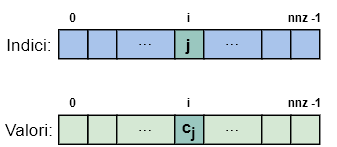
\includegraphics[scale=0.5]{Images/lazy_constraints} 
  \caption{\footnotesize{Array lazy constraints}}
  \label{lazy_constraints} 
\end{center} 
\end{figure}
\subsection{Lazy Constraint Callback}
Per poter utilizzare una lazy constraint callback, precedentemente implementata, all'interno del programma, prima di tutto è necessario installarla. Questo viene fatto attraverso la seguente funzione:
\begin{center}
\begin{tabular}{c}
\begin{lstlisting}[linewidth=385pt, basicstyle=\footnotesize\sffamily,] 
int CPXsetlazyconstraintcallbackfunc( CPXENVptr env,
		int(CPXPUBLIC *lazyconcallback)(CALLBACK_CUT_ARGS), void * cbhandle);    
\end{lstlisting}
\end{tabular}
\end{center}
\begin{table}[h]
\centering
\begin{tabular}{rl}
\textbf{env:} & {puntatore alla struttura ENV}\\
\textbf{lazyconcallback:} & {puntatore alla callback chiamata}\\
\textbf{cbhandle:} & {puntatore ad una struttura dati contenente le informazioni}\\
& {da passare alla callback}\\
\textbf{Return Value:} & {0 in caso di successo, un valore diverso da 0 se si verifica un errore}\\
\end{tabular}
\end{table}
Una volta installata la callback è necessario cambiare l'impostazione del numero di thread utilizzati dal programma. Infatti CPLEX, non sapendo se la funzione implementata dall'utente è thread safe, impedisce lo svolgimento di elaborazioni in parallelo con le callback. A meno che questo non venga esplicitamente dichiarato dall'utente con l'impostazione del corrispondente parametro.
Per questo può tornare utile la seguente funzione, che restituisce il numero di core presenti nel computer:\\
\begin{center}
\begin{tabular}{c}
\begin{lstlisting}[linewidth=280pt, basicstyle=\footnotesize\sffamily,]
int CPXgetnumcores(CPXCENVptr env, int * numcores_p); 
\end{lstlisting}
\end{tabular}
\end{center}
\begin{table}[h]
\centering
\begin{tabular}{rl}
\textbf{env:} & {puntatore ad una struttura ENV}\\
\textbf{numcores\_p:} & {puntatore alla variabile in cui scrivere il numero di core}\\ 
\textbf{Return Value:} & {0 in caso di successo, un valore diverso da 0 se si verifica un errore}\\           
\end{tabular}
\end{table} 
Come descritto nella sezione dedicata, le callback sono funzioni lasciate appositamente vuote da CPLEX, affinché l'utente possa implementarle in maniera personalizzata. Hanno però una dichiarazione standard, qui riportata: 
\begin{center}
\begin{lstlisting}[linewidth=400pt, basicstyle=\footnotesize\sffamily,]     
static int CPXPUBLIC name_function(CPXCENVptr env, void* cbdata, int wherefrom,
		 void* cbhandle, int* useraction_p);
\end{lstlisting}
\end{center}
\begin{table}[h]
\centering
\begin{tabular}{rl}
\textbf{env:} & {puntatore una struttura ENV}\\
\textbf{cbdata:} & {puntatore che contiene specifiche informazioni per la callback}\\
\textbf{wherefrom:} & {contiene dove è stata invocata la callback durante l'ottimizzazione} \\ 
\textbf{cbhandle:} & {puntatore a dati privati dell'utente} \\
\textbf{useraction\_p:} & {specifica le azioni da eseguire al termine della callback:}\\
& {CPX\_CALLBACK\_DEFAULT: usa il nodo di CPLEX selezionato}\\
& {CPX\_CALLBACK\_FAIL: esci dell'ottimizzazione}\\
& {CPX\_CALLBACK\_SET: usa il nodo selezionato come definito}\\  
& {nel valore di ritorno}\\ 
\textbf{Return Value:} & {0 in caso di successo, un valore diverso da 0 se si verifica un errore}\\                      
\end{tabular}
\end{table} 
Nell'implementarla bisogna fare particolare attenzione a renderla thread safe, se si vuole utilizzarla su più processi in parallelo. Infatti, nel caso in cui il programma lavorasse contemporaneamente con più processori, non si devono verificare interferenze di accesso agli stessi dati da parte di invocazioni diverse della callback. Quest'aspetto è lasciato a completa gestione dell'utente.\\
%CONTROLLARE COSA VUOL DIRE CPXPUBLIC
Per avere accesso alle variabili utilizzate dal nodo che invoca la callback è possibile chiamare la seguente funzione:
\begin{center}
\begin{tabular}{c}
\begin{lstlisting}[linewidth=410pt, basicstyle=\footnotesize\sffamily,]     
int CPXgetcallbacknodex(CPXCENVptr env, void * cbdata, int wherefrom, double * x, 
		int begin, int end);
\end{lstlisting}
\end{tabular}
\end{center}
\begin{table}[h]
\centering
\begin{tabular}{rl}
\textbf{env:} & {puntatore una struttura ENV}\\
\textbf{cbdata:} & {puntatore che contiene specifiche informazioni per la callback}\\
\textbf{wherefrom:} & {contiene in che punto dell'ottimizzazione è stata invocata la callback} \\ 
\textbf{x:} & {vettore in cui memorizzare le variabili} \\
\textbf{begin} & {indice della prima variabile che si vuole venga restituita}\\
\textbf{end} & {indice dell'ultima variabile che si vuole venga restituita}\\  
\textbf{Return Value:} & {0 in caso di successo, un valore diverso da 0 se si verifica un errore}\\                               
\end{tabular}
\end{table}
Invece, per ottenere informazioni riguardanti il problema di ottimizzazione che si sta risolvendo all'interno di una callback implementata dall'utente, è possibile utilizzare:
\begin{center}
\begin{tabular}{c}
\begin{lstlisting}[linewidth=415pt, basicstyle=\footnotesize\sffamily,]  
int CPXgetcallbackinfo(CPXCENVptr env, void * cbdata, int wherefrom, int whichinfo, 
		void * result_p);
\end{lstlisting}
\end{tabular}
\end{center}
\begin{table}[h]
\centering
\begin{tabular}{rl}
\textbf{env:} & {puntatore ad una struttura ENV}\\
\textbf{cbdata:} & {puntatore che contiene specifiche informazioni per la callback}\\
\textbf{wherefrom:} & {contiene in che punto dell'ottimizzazione è stata invocata la callback}\\ 
\textbf{whichinfo:} & {macro che specifica l'informazione che si desidera conoscere} \\
\textbf{result\_p:} & {puntatore di tipo void in cui verrà memorizzata l'informazione richiesta}\\ 
\textbf{Return Value:} & {0 in caso di successo, un valore diverso da 0 se si verifica un errore}\\          
\end{tabular}
\end{table}
Macro utili da utilizzare come parametro \textit{whichinfo} possono essere:
\begin{table}[h]
\centering \footnotesize
\begin{tabular}{|r|l|}
\hline
\textbf{CPX\_CALLBACK\_INFO\_MY\_THREAD\_NUM:} & {identifica il thread che }\\
&{ha eseguito la chiamata}\\
\hline
\textbf{CPX\_CALLBACK\_INFO\_BEST\_INTEGER:} & {valore della miglior}\\
&{soluzione intera}\\
\hline
\end{tabular}
\end{table}
\\Per conoscere il valore della funzione obiettivo del problema legato al nodo corrente che invoca la callback:
\begin{center}
\begin{tabular}{c}
\begin{lstlisting}[linewidth=380pt, basicstyle=\footnotesize\sffamily,] 
int CPXgetcallbacknodeobjval(CPXCENVptr env, void * cbdata, int wherefrom, 
		double * objval_p); 
\end{lstlisting}
\end{tabular}
\end{center}
\begin{table}[H]
\centering
\begin{tabular}{rl}
\textbf{env:} & {puntatore ad una struttura ENV}\\
\textbf{cbdata:} & {puntatore che contiene specifiche informazioni per la callback}\\
\textbf{wherefrom:} & {contiene in che punto dell'ottimizzazione è stata invocata la callback} \\ 
\textbf{objval\_p:} & {puntatore ad una variabile in cui memorizzare il costo} \\
\textbf{Return Value:} & {0 in caso di successo, un valore diverso da 0 se si verifica un errore}\\  
\end{tabular}
\end{table}
All'interno della lazy callback è necessario aggiungere il taglio voluto al nodo corrente che la invoca. Questo può essere fatto in due diverse modalità: globale o locale.\\
Nel primo caso il vincolo aggiunto sarà visibile da tutti i nodi. Inoltre, in caso non lo ritenga più necessario, CPLEX potrà eliminarlo dal modello. Quest'operazione viene detta \textit{purge} e si verifica, ad esempio, quando un taglio non viene applicato per molte iterazioni consecutive. Per un vincolo globale viene chiamata la seguente funzione, che ne aggiunge uno alla volta:
\begin{center}
\begin{tabular}{c}
\begin{lstlisting}[linewidth=400pt, basicstyle=\footnotesize\sffamily,]  
int CPXcutcallbackadd( CPXCENVptr env, void * cbdata, int wherefrom, int nzcnt, 
		double rhs, int sense, int const * cutind, double const * cutval, 
		int purgeable );
\end{lstlisting}
\end{tabular}
\end{center}
\begin{table}[H]
\centering
\begin{tabular}{rl}
\textbf{env:} & {puntatore ad una struttura ENV}\\
\textbf{cbdata:} & {puntatore che contiene specifiche informazioni per la callback}\\
\textbf{wherefrom:} & {contiene in che punto dell'ottimizzazione è stata invocata la callback} \\ 
\textbf{nzcnt:} & {numero di coefficienti non nulli} \\
\textbf{rhs:} & {valore del termine noto} \\
\textbf{sense:} & {tipologia del taglio da aggiungere, a scelta tra} \\
&{\textit{'L'} per vincolo $\leq$}\\
&{\textit{'E'} per vincolo $=$}\\
&{\textit{'G'} per vincolo $\geq$}\\
\textbf{cutind:} & {vettore contente gli indici dei coefficienti del taglio} \\
\textbf{cutval:} & {vettore contenente i coefficienti delle variabili nel taglio} \\
\textbf{purgeable:} & {intero che specifica in che modo CPLEX deve trattare il taglio, consigliato 0} \\
\textbf{Return Value:} & {0 in caso di successo, un valore diverso da 0 se si verifica un errore}\\  
\end{tabular}
\end{table}
Nella seconda modalità, locale, il taglio aggiunto sarà visibile solo ai nodi discendenti di quello che invoca la callback. Viene implementata con la seguente chiamata:
\begin{center}
\begin{tabular}{c}
\begin{lstlisting}[linewidth=400pt, basicstyle=\footnotesize\sffamily,] 
int CPXcutcallbackaddlocal( CPXCENVptrenv, void *cbdata, int wherefrom, 
		int nzcnt, double rhs, int sense, int const *cutind, double const *cutval ); 
\end{lstlisting}
\end{tabular}
\end{center}
\begin{table}[h]
\centering
\begin{tabular}{rl}
\textbf{env:} & {puntatore ad una struttura ENV}\\
\textbf{cbdata:} & {puntatore che contiene specifiche informazioni per la callback}\\
\textbf{wherefrom:} & {contiene in che punto dell'ottimizzazione è stata invocata la callback} \\ 
\textbf{nzcnt:} & {numero di coefficienti non nulli} \\
\textbf{rhs:} & {valore del termine noto} \\
\textbf{sense:} & {tipologia del taglio da aggiungere, a scelta tra} \\
&{\textit{'L'} per vincolo $\leq$}\\
&{\textit{'E'} per vincolo $=$}\\
&{\textit{'G'} per vincolo $\geq$}\\
\textbf{cutind:} & {vettore contente gli indici dei coefficienti del taglio} \\
\textbf{cutval:} & {vettore contenente i coefficienti delle variabili nel taglio} \\
\textbf{Return Value:} & {0 in caso di successo, un valore diverso da 0 se si verifica un errore}\\ 
\end{tabular}
\end{table}
\subsection{Heuristic Callback}
Per poter suggerire a CPLEX una soluzione del problema in esame calcolata dall'utente, è necessario utilizzare un particolare tipo di callback, detta \textit{heuristic callback}. Questa, dopo essere stata installata, verrà invocata ad ogni nodo dell'albero del branch and cut.\\
Per installare la callback viene utilizzata la seguente funzione:
\begin{center}
\begin{tabular}{c}
\begin{lstlisting}[linewidth=330pt, basicstyle=\footnotesize\sffamily,]    
int CPXsetheuristiccallbackfunc(CPXENVptr env,
		 int(CPXPUBLIC *heuristiccallback)(CALLBACK_HEURISTIC_ARGS), 
		 void * cbhandle);
\end{lstlisting}
\end{tabular}
\end{center}
\begin{table}[h]
\centering
\begin{tabular}{rl}
\textbf{env:} & {puntatore ad una struttura ENV}\\
\textbf{heuristiccallback:} & {puntatore all'heuristic callback scritta dall'utente}\\
\textbf{cbhandle:} & {puntatore a dati privati dell'utente}\\
\textbf{Return Value:} & {0 in caso di successo, un valore diverso da 0 se si verifica un errore}\\
\end{tabular}
\end{table}
La callback dell'utente deve avere la dichiarazione specificata di seguito:
\begin{center}
\begin{tabular}{c}
\begin{lstlisting}[linewidth=382pt, basicstyle=\footnotesize\sffamily,] 
 int callback (CPXCENVptr env, void *cbdata, int wherefrom, void *cbhandle, 
 		double *objval_p, double *x, int *checkfeas_p, int *useraction_p);
\end{lstlisting}
\end{tabular}
\end{center}
\begin{table}[h]
\centering
\begin{tabular}{rl}
\textbf{env:} & {puntatore ad una struttura ENV}\\
\textbf{cbdata:} & {puntatore che contiene specifiche informazioni per la callback}\\
\textbf{wherefrom:} & {contiene in che punto dell'ottimizzazione è stata invocata la callback} \\ 
\textbf{cbhandle:} & {puntatore a dati privati dell'utente}\\
\textbf{objval\_p:} & {puntatore ad una variabile che in ingresso contiene il valore della funzione}\\
&{ obiettivo del problema e in uscita il valore della funzione obiettivo trovata}\\
&{nella funzione stessa, se esiste}\\
\textbf{x:} & {vettore che in ingresso contiene una soluzione valida per il problema }\\
&{e in uscita i valori della soluzione trovata nella funzione, se presente}\\
\textbf{checkfeas\_p:} & {puntatore che specifica se CPLEX deve verificare la soluzione trovata}\\
&{oppure no}\\
\textbf{useraction\_p:} & {puntatore ad un intero che specifica a CPLEX come proseguire la }\\
&{computazione al termine della callback dell'utente, scelto tra:}\\
&{\textit{CPX\_CALLBACK\_DEFAULT}: nessuna soluzione trovata}\\
&{\textit{CPX\_CALLBACK\_FAIL}: uscire dall'ottimizzazione}\\
&{\textit{CPX\_CALLBACK\_SET}: usare la soluzione fornita dall'utente}\\
\textbf{Return Value:} & {0 in caso di successo, un valore diverso da 0 se si verifica un errore}\\
\end{tabular}
\end{table}

\subsection{Generic Callback}% cambiare titolo da Lazy Constraint Callback General a general callback
Per evitare che alcune procedure interne a CPLEX vengano disattivate nel momento dell'installazione di una callback, recentemente ne è stata sviluppata una particolare tipologia, detta \textit{generic}. Questa non è relativa a una specifica versione di callback, come quelle descritte nelle sezioni precedenti, ma può essere invocata in contesti diversi e con diversi scopi.\\
Per installare una generic callback viene utilizzata la seguente funzione, in cui  è necessario specificare il contesto in cui invocare la callback:
\vspace{1 cm}
\begin{center}
\begin{tabular}{c}
\begin{lstlisting}[linewidth=380pt, basicstyle=\footnotesize\sffamily,]    
int CPXcallbacksetfunc ( CPXENVptr env, CPXLPptr lp, CPXLONG contextmask, 
		CPXCALLBACKFUNC *callback, void * userhandle );
\end{lstlisting}
\end{tabular}
\end{center}
\begin{table}[h]
\centering
\begin{tabular}{rl}
\textbf{env:} & {puntatore ad una struttura ENV}\\
\textbf{lp:} & {puntatore alla struttura LP}\\
\textbf{contextmask:} & {specifica in quali contesti deve essere invocata la callback, è possibile }\\
&{metterne in or anche più di uno e gestire poi i singoli casi dall'interno}\\
&{della funzione}\\
\textbf{callback:} & {puntatore alla callback scritta dall'utente} \\
\textbf{userhandle:} & {puntatore ad una struttura che contiene i dati da passare alla callback} \\
\textbf{Return Value:} & {0 in caso di successo, un valore diverso da 0 se si verifica un errore}\\
\end{tabular}
\end{table}
Il parametro \textit{contextmask} può variare a seconda dello scopo della callback creata. Alcuni possibili valori sono:
\begin{itemize}
\item{\textbf{CPX\_CALLBACKCONTEXT\_CANDIDATE}:\\la callback verrà invocata quando viene trovata da CPLEX una nuova soluzione possibile che l'utente potrà rifiutare;}
\item{\textbf{CPX\_CALLBACKCONTEXT\_LOCAL\_PROGRESS}: \\la callback verrà invocata nel momento in cui un thread effettua un progresso, non ancora noto globalmente, nella soluzione del problema. In questo contesto l'utente può suggerire a CPLEX una soluzione da cui proseguire la computazione (analogamente alle heuristic callback).}\\
\end{itemize}
L'utente può specificare più contesti con una sola installazione, è sufficiente separare le macro desiderate con l'operatore or bitwise ('|').\\
La user-callback implementata deve avere questa dichiarazione:
\begin{center}
\begin{tabular}{c}
\begin{lstlisting}[linewidth=350pt, basicstyle=\footnotesize\sffamily,]    
static int CPXPUBLIC name_general_callback(CPXCALLBACKCONTEXTptr
                     context, CPXLONG contextid, void* userhandle);
\end{lstlisting}
\end{tabular}
\end{center}
\begin{table}[h]
\centering
\begin{tabular}{rl}
\textbf{contex:} & {puntatore ad una struttura di contesto della callback}\\
%opaque callback context structure, verificare traduzione
\textbf{contextid:} & {intero che specifica il contesto in cui viene invocata la callback}\\
\textbf{userhandle:} & {argomento passato alla callback nell'installazione}\\
\textbf{Return Value:} & {0 in caso di successo, un valore diverso da 0 se si verifica un errore}\\
\end{tabular}
\end{table}
L'utente può installare una sola user-callback, ma al suo interno può distinguere il contesto in cui è stata invocata grazie al parametro \textit{contextid}.\\
Per poter accedere alla soluzione candidata e al suo costo, deve essere presente la seguente chiamata, che è specifica per il contesto \textbf{CPX\_CALLBACKCONTEXT\_CANDIDATE}:
\begin{center}
\begin{tabular}{c}
\begin{lstlisting}[linewidth=380pt, basicstyle=\footnotesize\sffamily,]
int CPXcallbackgetcandidatepoint( CPXCALLBACKCONTEXptr context, double *x, 
		CPXDIM begin, CPXDIM end, double *obj_p, );    
\end{lstlisting}
\end{tabular}
\end{center}
\begin{table}[h]
\centering
\begin{tabular}{rl}
\textbf{contex:} & {contesto, come passato alla callback scritta dall'utente}\\
\textbf{x:} & {vettore dove memorizzare i valori richiesti}\\
\textbf{begin:} & {indice prima colonna richiesta}\\
\textbf{end:} & {indice dell'ultima colonna richiesta}\\
\end{tabular}
\end{table}
\begin{table}[h]
\centering
\begin{tabular}{rl}
\textbf{obi\_p:} & {buffer in cui memorizzare il costo della soluzione candidata,}\\
&{può essere NULL}\\
\textbf{Return Value:} & {0 in caso di successo, un valore diverso da 0 se si verifica un errore}\\
\end{tabular}
\end{table}
Per poter scartare una soluzione, nel caso in cui violi alcuni tagli specificati nella chiamata stessa, viene utilizzata la seguente funzione. Anche questa è specifica per il contesto 
\\\textbf{CPX\_CALLBACKCONTEXT\_CANDIDATE}.
\begin{center}
\begin{tabular}{c}
\begin{lstlisting}[linewidth=420pt, basicstyle=\footnotesize\sffamily,] 
int CPXcallbackrejectcandidate( CPXCALLBACKCONTEXTptr context, int rcnt, int nzcnt, 
		double const *rhs, char const *sense, int const *rmatbeg, int const *rmatind, 
		double const *rmatval );   
\end{lstlisting}
\end{tabular}
\end{center}
\begin{table}[h]
\centering
\begin{tabular}{rl}
\textbf{contex:} & {contesto, come passato alla callback scritta dall'utente}\\
\textbf{rcnt:} & {numero di vincoli che tagliano la soluzione}\\
\textbf{nzcnt:} & {numero di coefficienti non nulli nel vincolo}\\
\textbf{rhs:} & {vettore di termini noti}\\
\textbf{sense:} & {vettore con la tipologia dei vincoli specificati}\\
\textbf{rmatbeg:} & {vettore di indici che specifica dove inizia ogni vincolo}\\
\textbf{rmatind:} & {vettore di indici delle colonne con coefficienti non nulli}\\
\textbf{rmatval:} & {coefficienti non nulli delle colonne specificate}\\
\textbf{Return Value:} & {0 in caso di successo, un valore diverso da 0 se si verifica un errore}\\
\end{tabular}
\end{table}
Per suggerire a CPLEX la soluzione da cui proseguire nella computazione dev'essere utilizzata la funzione:
\begin{center}
\begin{tabular}{c}
\begin{lstlisting}[linewidth=365pt, basicstyle=\footnotesize\sffamily,]
int CPXcallbackpostheursoln( CPXCALLBACKCONTEXTptr context, CPXDIM cnt, 
			CPXDIM const * ind, double const * val, double obj, 
			CPXCALLBACKSOLUTIONSTRATEGY strat );    
\end{lstlisting}
\end{tabular}
\end{center}
\begin{table}[h]
\centering
\begin{tabular}{rl}
\textbf{contex:} & {contesto, come passato alla callback scritta dall'utente}\\
\textbf{cnt:} & {numero di elementi nei vettori ind e val}\\
\textbf{ind:} & {vettore di indici non nulli dei valori della soluzione}\\
\textbf{val:} & {vettore di valori non nulli della soluzione, possono essere NaN nel caso in cui }\\
&{la soluzione sia parziale}\\
\textbf{obj:} & {costo della nuova soluzione}\\
\textbf{strat:} & {strategia con cui CPLEX deve completare la nuova soluzione, nel caso sia }\\
&{parziale, scelta tra:}\\
&{\textit{CPXCALLBACKSOLUTION\_NOCHECK} affinchè CPLEX}\\ 
&{non controlli l'attuabilità della soluzione (che deve essere completa) }\\
&{\textit{CPXCALLBACKSOLUTION\_CHECKFEAS} affinchè CPLEX}\\
&{controlli solamente se la soluzione è attuabile (la soluzione proposta }\\
&{deve essere completa)}\\
&{\textit{CPXCALLBACKSOLUTION\_PROPAGATE} affinchè CPLEX }\\
\end{tabular}
\end{table}
\begin{table}[h]
\centering
\begin{tabular}{rl}
&{cerchi di completare la soluzione attraverso la propagazione del bound}\\
&{\textit{CPXCALLBACKSOLUTION\_SOLVE} affinchè CPLEX}\\ 
&{fissi le variabili specificate nella soluzione e cerchi di risolvere il risultante }\\
&{problema ridotto}\\
\textbf{Return Value:} & {0 in caso di successo, un valore diverso da 0 se si verifica un errore}\\
\end{tabular}
\end{table}
CPLEX utilizzerà la soluzione proposta dall'utente solo nel caso in cui questa abbia costo inferiore all'incumbent.
\section{Parametri}\label{param}
Con le seguenti funzioni è possibile modificare i parametri di configurazione di CPLEX, altrimenti impostati ai valori di default.
Nel caso in cui si tratti di parametri di tipo INT è necessario invocare:\\
\begin{center}
\begin{tabular}{c}
\begin{lstlisting}[linewidth=330pt, basicstyle=\footnotesize\sffamily,]     
int CPXsetintparam(CPXENVptr env, int whichparam, int newvalue);
\end{lstlisting}
\end{tabular}
\end{center}
mentre se di tipo DOUBLE:\\
\begin{center}
\begin{tabular}{c}
\begin{lstlisting}[linewidth=340pt, basicstyle=\footnotesize\sffamily,]  
int CPXsetdblparam(CPXENVptr env, int whichparam, double newvalue);
\end{lstlisting}
\end{tabular}
\end{center}
In entrambe le funzioni:
\begin{table}[h]
\centering
\begin{tabular}{rl}
\textbf{env:} & {puntatore alla struttura ENV di cui si vogliono cambiare i parametri}\\
\textbf{whichparam:} & {intero corrispondente al parametro da modificare (vedi Tabella \ref{param_table})}\\
\textbf{newvalue:} & {nuovo valore (rispettivamente intero o double) del parametro}\\
\textbf{Return Value:} & {0 in caso di successo, un valore diverso da 0 se si verifica un errore}\\
\end{tabular}
\end{table}
\begin{table}[h]
\centering\footnotesize
\begin{tabular}{|l|l|}
\hline
\multirow{2}{*}{\textbf{CPX\_PARAM\_EPGAP}} & {tolleranza dell'intervallo tra la migliore funzione obiettivo intera}\\
& { e la funzione obiettivo del miglior nodo rimanente.}\\
\hline
\multirow{3}{*}{\textbf{CPX\_PARAM\_NODELIM}} & {massimo numero di nodi da risolvere prima che l'algoritmo}\\
& { termini senza aver aggiunto l'ottimalità}\\
& {(0 impone di fermarsi alla radice).}\\
\hline
\multirow{2}{*}{\textbf{CPX\_PARAM\_POPULATELIM}} & {limita il numero di soluzioni MIP generate per il pool  }\\
& {di soluzioni durante ogni chiamata alla procedura populate.}\\
\hline
\textbf{CPX\_PARAM\_SCRIND} & {visione o meno dei messaggi di log di CPLEX.}\\
\hline
\textbf{CPX\_PARAM\_MIPCBREDLP} & {permette, dalla callback chiamata, di accedere  }\\
&{al modello originale del problema e non a quello ridotto .}\\
\hline
\textbf{CPX\_PARAM\_THREADS} & {imposta il numero massimo di thread utilizzabili. }\\
\hline
\textbf{CPX\_PARAM\_RINSHEUR} & {imposta la frequenza (ogni quanti nodi) con cui deve}\\
&{essere invocato da CPLEX l'algoritmo euristico Rins.}\\
\hline
\textbf{CPX\_PARAM\_POLISHTIME} & {imposta quanto tempo in secondi deve dedicare CPLEX}\\
&{a fare il polish della soluzione.}\\
\hline
\end{tabular}
\end{table}
\begin{table}[h]
\centering\footnotesize
\begin{tabular}{|l|l|}
\hline
\textbf{CPX\_PARAM\_INTSOLLIM}&{imposta il numero di soluzioni MIP da trovare prima di fermarsi.}\\
\hline
\textbf{CPX\_PARAM\_TIMELIMIT}&{imposta il tempo massimo per il calcolo della soluzione.}\\
\hline
\textbf{CPX\_PARAM\_RANDOMSEED}&{imposta il random seed.}\\
\hline
\end{tabular}
\caption{Parametri.}\label{param_table}
\end{table}
\vspace{2 cm}
\section{Costanti utili}
Di seguito sono riportate alcune macro utili di CPLEX, insieme ai loro corrispondenti valori:
\begin{table}[h]
\footnotesize\centering
\begin{tabular}{|r|l|}
\hline
\textbf{CPX\_ON} & {\textbf{1}}\\
{} & {valore da assegnare ad alcuni parametri per abilitarli}\\
\hline
\textbf{CPX\_OFF} & {0}\\
{} & {valore da assegnare ad alcuni parametri per disabilitarli}\\
\hline
\textbf{CPX\_INFBOUND} & {$+\infty$}\\
{} & {massimo valore intero utilizzabile in CPLEX}\\
\hline
\end{tabular}
\end{table}

\chapter{Gnuplot}\label{gnuplot}
Nella nostra implementazione, una volta ottenuta la soluzione del problema di ottimizzazione, ne viene disegnato il grafo per facilitare all'utente la comprensione della sua correttezza. Per fare ciò viene sfruttato GNUplot, un programma di tipo command-driven.\\
Per poterlo utilizzare all'interno del proprio programma esistono due metodi:
\begin{itemize}
\item{Collegare la libreria ed invocare le sue funzioni all'interno del programma}
\item{Collegare l'eseguibile interattivo al proprio programma. In questo caso i comandi deve essere passati all'eseguibile attraverso un file di testo e l'utilizzo di un pipe.}\\
\end{itemize}
In questa trattazione è stato scelto il secondo metodo. All'interno del file è possibile specificare a Gnuplot le caratteristiche grafiche che deve aver il grafo. Di seguito viene riportato un esempio di tale file.\\

\lstinputlisting[caption={\footnotesize{style.txt}}, style=code, firstnumber=1, firstline=1, lastline=12, label=style_example]{Source/style_example.txt}

Nell'esempio sopra riportato, nella prima parte viene definito lo stile, il colore delle linee e la tipologia di punti, che verrano in seguito visualizzati all'interno del grafico prodotto.\\In seguito viene effettuato il plot del grafo in una finestra, utilizzando il primo e secondo valore di ciascuna riga del file \textbf{solution.dat} come coordinate mentre il terzo valore viene utilizzato come etichetta.\\\\
Il file \textbf{solution.dat} contiene le informazioni relative alla soluzione del grafico in cui ciascuna riga ha la seguente forma:
\begin{center}
\begin{tabular}{c}
\begin{lstlisting}[linewidth=290pt,basicstyle=\footnotesize\sffamily,]     
coordinata_x   coordinata_y   posizione_in_tour
\end{lstlisting}
\end{tabular}
\end{center}
\textbf{coordinata\_x} rappresenta la coordinata x del nodo;\\
\textbf{coordinata\_y} rappresenta la coordinata y del nodo;\\
\textbf{posizione\_in\_tour} rappresenta l'ordine del nodo all'interno del tour, assunto come nodo di origine il nodo 1.\\\\
Il grafico viene generato dal comando \textbf{plot}, leggendo tutte le righe non vuote e disegnando un punto nella posizione \textbf{(coordinata\_x, coordinata\_y)} del grafico 2D. In seguito viene tracciata una linea solo tra coppie di punti legati a righe consecutive non vuote all'interno di \textbf{solution.dat}.\\\\
Attraverso le istruzioni riportate nelle righe 10-12 di \textbf{style.txt}, viene invece salvato il grafico appena generato nell'immagine \textbf{solution.png}.\\\\
Di seguito vengono riportate le varie fasi necessarie alla definizione di un pipe e al passaggio di questo al programma GNUplot:
\begin{itemize}
\item{\textbf{Definizione del pipe}
\lstinputlisting[style=code, firstnumber=1, firstline=1, lastline=1, label=style_example language=C]{Source/gnuplotC.txt}
dove \textbf{GNUPLOT\_EXE} è una stringa composta dal percorso completo dell'eseguibile di GNUplot, seguita dall'argomento \textbf{-persistent} (es. \textit{"D:/Programs/GNUplot/bin/gnuplot -persistent"}).
}
\item{\textbf{Passaggio delle istruzioni a GNUplot}
\lstinputlisting[style=code, firstnumber=2, firstline=2, lastline=10, label=style_example, language=C]{Source/gnuplotC.txt}
viene passata una riga alla volta, del file \textbf{style.txt}, a GNUplot mediante il pipe precedentemente creato.
}
\item{\textbf{Chiusura del pipe}
\lstinputlisting[style=code, firstnumber=11, firstline=11, lastline=11, label=style_example, language=C]{Source/gnuplotC.txt}
}
\end{itemize}
\chapter{Performance profile in python}\label{perf_profile_py}
Il programma utilizzato per la creazione del performance profile dei diversi algoritmo è perprof.py\cite{salvagnin_perf}. Di seguito vengono riportati i principali argomenti da linea di comando che possono essere utilizzati:

\begin{table}[h]
\centering
\begin{tabular}{|r|l|}
\hline
\textbf{-D delimiter} & {specifica che delimiter verrà usato come separatore tra le}\\
& {parole in una riga}\\
\hline
\textbf{-M value} & {imposta value come il massimo valore di ratio (asse x)}\\
\hline
\textbf{-S value} & {value rappresenta la quantità che viene sommata a}\\
& {ciascun tempo di esecuzione prima del confronto.}\\
& {Questo parametro è utile per non enfatizzare troppo}\\
& {le differenze di pochi ms tra gli algoritmi.}\\
\hline
\textbf{-L} & {stampa in scala logaritmica}\\
\hline
\textbf{-T value} & {nel file passato al programma, il TIME LIMIT= value}\\
\hline
\textbf{-P "title"} & {title è il titolo del plot}\\
\hline
\textbf{-X value} & {nome dell'asse x (default ='Time Ratio')}\\
\hline
\textbf{-B} & {plot in bianco e nero}\\
\hline
\end{tabular}
\end{table}
Di seguito viene riportato un esempio dell'esecuzione del programma, del suo input e del suo output:
\begin{itemize}
\item{\textbf{comando}
\begin{center}
\begin{tabular}{c}
\begin{lstlisting}[linewidth=330pt, basicstyle=\footnotesize\sffamily,] 
python perfprof.py -D , -T 3600 -S 2 -M 20 esempio.csv out.pdf
		-P "all instances, shift 2 sec.s"
\end{lstlisting}
\end{tabular}
\end{center}
}
\item{\textbf{file di input con i dati}\\
Viene riportato parte del contenuto di esempio.csv .
\begin{center}
\begin{tabular}{c}
\begin{lstlisting}[linewidth=240pt, basicstyle=\footnotesize\sffamily,] 
3, Alg1, Alg2, Alg3
model_1.lp, 2.696693, 3.272468, 2.434147
model_2.lp, 0.407689, 1.631921, 1.198957
model_3.lp, 0.333669, 0.432553, 0.966638
\end{lstlisting}
\end{tabular}
\end{center}
La prima riga deve necessariamente contenere in ordine il numero di algoritmi analizzati e i loro nomi. Nelle righe seguenti viene riportato invece il nome del file lp e i tempi di esecuzione elencati secondo la sequenza di algoritmi specificata all'inizio.
Ogni campo di ciascuna riga deve essere separato dal delimitatore specificato all'avvio del programma attraverso l'opzione -D.
}
\item{\textbf{immagine di output}\\
Il grafico viene restituito nel file out.pdf specificato da linea di comando chiamando il programma.
\begin{figure}[h] 
\begin{center} 
  % Requires \usepackage{graphicx} 
  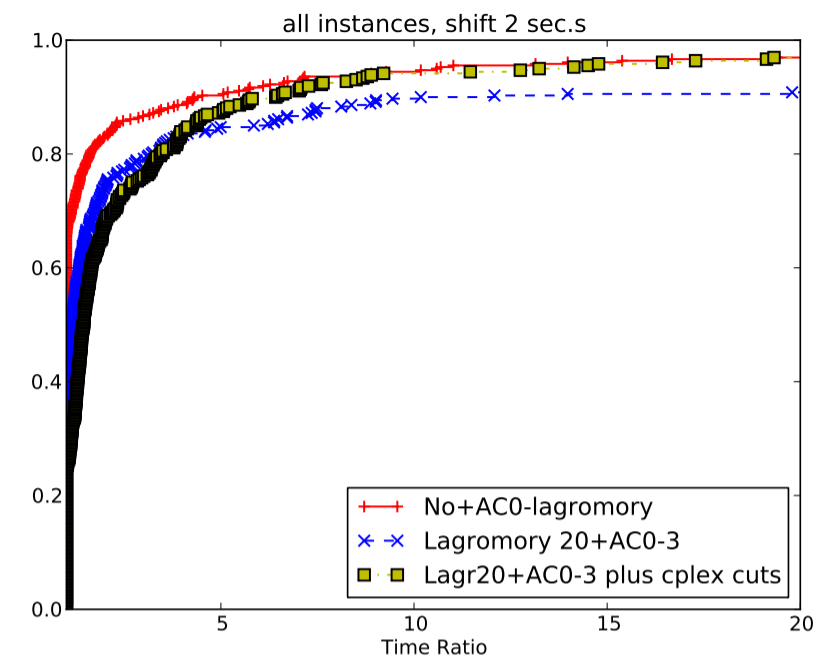
\includegraphics[scale=0.6]{Images/profile_out}\\ 
\end{center} 
\end{figure}
}
\end{itemize}
%Bibliografia
\addcontentsline{toc}{chapter}{Bibliografia}
\bibliographystyle{plain}
\renewcommand{\bibname}{Bibliografia}
\bibliography{Chapters/biblio}

\end{document}